\documentclass[a4paper,12pt,twoside]{article}
\usepackage{amsmath}
\usepackage{amssymb}
\usepackage{bm}
\usepackage{booktabs}
\usepackage[small,bf]{caption}
\usepackage{comment}
\usepackage{cuted}
\usepackage[shortlabels]{enumitem}
\usepackage{fancyhdr}
\usepackage{fancybox}
\usepackage{float}
\usepackage[T1]{fontenc}
\usepackage[a4paper,left=1in,right=1in,top=0.25in,bottom=1in,
    headheight=76.33466pt,
    headsep=\dimexpr1in-62.33466pt\relax,
    includehead
]{geometry}
\usepackage{graphicx}
\usepackage{hyperref}
\usepackage[utf8]{inputenc}
% \usepackage{lipsum}
\usepackage{listings}
\usepackage{minted}
\usemintedstyle{emacs}
\usepackage{multirow}
\usepackage{parskip}
\usepackage{ragged2e}
\usepackage{setspace}
\usepackage{soul}
% \onehalfspacing
\usepackage{subcaption}
% \usepackage[subrefformat=parens,labelformat=parens]{subfig}
\usepackage{tabularx}
% \usepackage{titling}
\usepackage{xurl}
\usepackage{biblatex}
\addbibresource{Lab5.bib}
\usepackage{background}
\backgroundsetup{contents=
\includegraphics{waterprint.jpg}, scale=0.8, opacity=0.1}
\pagestyle{fancy}
\fancyhf{}
\fancyhead[LE,RO]{}
\fancyhead[CE,CO]{
\includegraphics[width=0.7\textwidth]{JILogo.png}}
\fancyhead[RE,LO]{}
\fancyfoot[CE,CO]{\leftmark}
\fancyfoot[CE,CO]{\thepage}
\lfoot{\textit{ECE4810J \textbf{SoC Design} | Fall 2022}}
\renewcommand{\headrulewidth}{1pt}
\renewcommand{\footrulewidth}{1pt}
\definecolor{caption2color}{HTML}{2e5395}
\hypersetup{
    colorlinks=true,
    linkcolor=blue,
    filecolor=magenta,      
    urlcolor=cyan,
    pdfpagemode=FullScreen,
}
\definecolor{codegreen}{rgb}{0,0.6,0}
\definecolor{codegray}{rgb}{0.5,0.5,0.5}
\definecolor{codepurple}{rgb}{0.58,0,0.82}
\definecolor{backcolour}{rgb}{0.95,0.95,0.92}

\lstdefinestyle{mystyle}{
    backgroundcolor=\color{backcolour},   
    commentstyle=\color{codegreen},
    keywordstyle=\color{magenta},
    numberstyle=\tiny\color{codegray},
    stringstyle=\color{codepurple},
    basicstyle=\ttfamily\footnotesize,
    breakatwhitespace=false,         
    breaklines=true,                 
    captionpos=b,                    
    keepspaces=true,                 
    numbers=left,                    
    numbersep=5pt,                  
    showspaces=false,                
    showstringspaces=false,
    showtabs=false,                  
    tabsize=2
}

\lstset{style=mystyle}

\usepackage[percent]{overpic}

\author{Yihua Liu}
\title{ECE4810J FA2021\\ \small Lab \#4}
\date{October 24, 2022}

\begin{document}
% \maketitle
\thispagestyle{fancy}

\begin{center}
    \vspace*{0pt}
    \Large{\textbf{ECE4810J SoC Design}}\\
    \vspace*{2pt}
    \large{Fall 2022}\\
    \vspace*{10pt}
    \Large{\textcolor{caption2color}{Lab \#5 ASIC Backend Flow}}\\
    \normalsize{\hl{Due: 11:59pm Nov. 6th, 2022}}
    \rule[-5pt]{.97\linewidth}{0.05em}
\end{center}

\textbf{Logistics:}
\begin{itemize}
    \item This lab is a team exercise.
    \item Please use the discussion board on Piazza for Q\&A.
    \item All reports and code (if available) MUST be submitted to the assignment of Canvas.
    \item Internet usage is allowed and encouraged.
    \item No late submission is allowed for this lab.
\end{itemize}

\tableofcontents

\newpage
\section{Overview}
In this lab, you will learn about ASIC design flow. The goals of this lab are to:
\begin{itemize}
    \item Learn how to compile the design with IC Compiler and what kind of commands are needed for it.
    \item Learn how to use Formality to detect unexpected differences that may have been introduced into a design during development.
    \item Learn how to use PrimeTime to validate the timing performance of a design by checking all possible paths for timing violations without using logic simulation or test vectors.
\end{itemize}

\section{Physical Design}\label{SPD}
\subsection{Introduction}
IC Compiler is a single, convergent netlist-to-GDSII synthesis design tool for chip designers developing very deep submicron designs. It takes as input a gate-level netlist, a detailed floorplan, timing constraints, physical and timing libraries, and foundry-process data, and it generates as output either a GDSII-format file of the layout.
IC Compiler provides two user interfaces:
\begin{itemize}
    \item Shell interface (icc\_shell) - The IC Compiler command-line interface is used for scripts, batch mode, and push-button operations.
    \item Graphical user interface (GUI) - The IC Compiler graphical user interface is an advanced analysis and physical editing tool.
\end{itemize}
\begin{figure}[H]
    \centering
    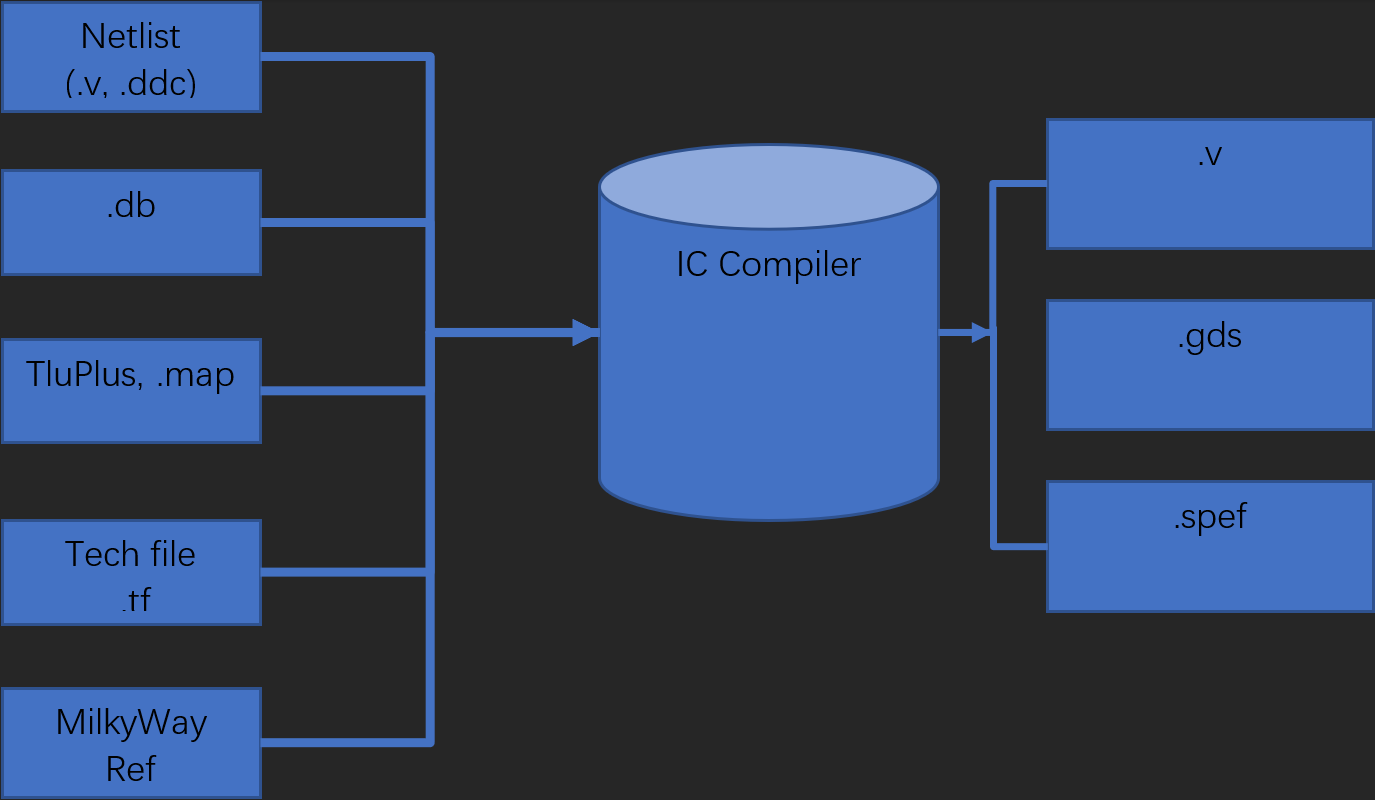
\includegraphics[width=0.9\textwidth]{images/1.png}
    \caption{Input and output files of IC compiler.}
\end{figure}
The cell logic, timing, and power information are typically contained in a set of Synopsys databases (.db).

\textbf{Tech file} - A technology file provides technology-specific information, such as the names and physical and electrical characteristics of each metal layer and the routing design rules. IC Compiler uses the Milkyway design library to access the technology information. A technology file contains process-specific data.
\textbf{TluPlus} - The parasitic attributes define the metal layer parasitics. In general, IC Compiler gets the parasitic information from the TLUPlus files rather than from the technology file.

% \textit{Synopsys IC Compiler has been moved to Synopsys IC Compiler II years ago; thus, we will use Synopsys IC Compiler II (icc2) Version R-2020.09-SP6 for linux64 in this lab. You can modify your \texttt{.cshrc} to launch the latest Synopsys IC Compiler II}.
\textit{We will use Synopsys IC Compiler Version Q-2019.12-SP5 for linux64 in this lab. You can modify your \texttt{.cshrc} to launch the latest Synopsys IC Compiler. However, we will sooner or later migrate to Synopsys IC Compiler II (icc2\_shell)}

Synopsys IC Compiler includes
\begin{itemize}
    \item IC Compiler (TM)
    \item IC Compiler-PC (TM)
    \item IC Compiler-XP (TM)
    \item IC Compiler-DP (TM)
    \item IC Compiler-AG (TM)
\end{itemize}
\subsection{Simplified IC Compiler Design Flow}\label{SICCFlow}
\begin{figure}[H]
    \centering
    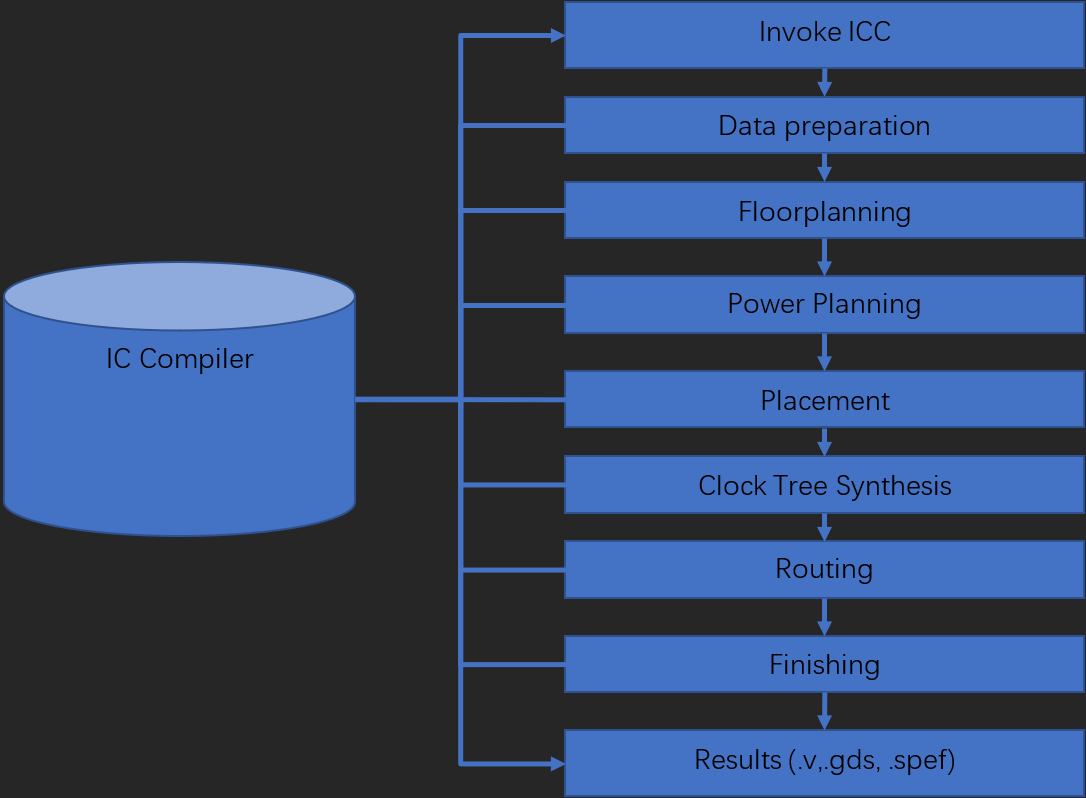
\includegraphics[width=0.8\textwidth]{images/2.png}
    \caption{Simplified IC Compiler Design Flow.}
\end{figure}
\begin{enumerate}
    \item Start IC Compiler graphical user interface (GUI) from the \textbf{work} directory. To start the IC Compiler command-line interface, enter the following commands at the UNIX or Linux prompt:
    \begin{minted}{bash}
unzip /home/Flow/Synopsys/Scripts/Icc32.zip -d ~/synopsys/syn_tut/
cd ~/synopsys/syn_tut/icc_32/work
icc_shell -gui
    \end{minted}
    This opens the IC Compiler top-level GUI window (Figure \ref{f3}).
    \begin{figure}[H]
        \centering
        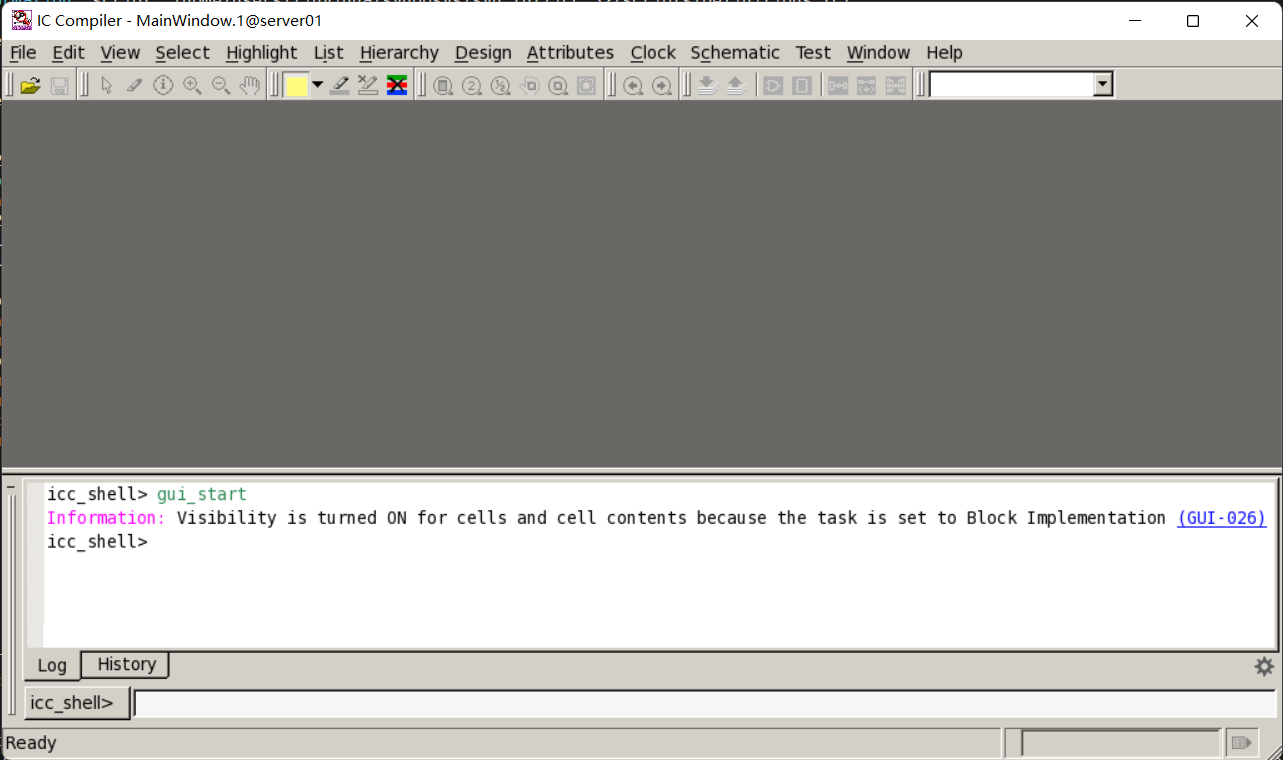
\includegraphics[width=0.8\textwidth]{images/3.png}
        \caption{IC Compiler Top-level GUI window.}
        \label{f3}
    \end{figure}
    % \textit{You can click the Console tab at the bottom to open the traditional Log and History views and double-click it to fix it}.\\
    The libraries are appended to the search path by running the setup.tcl script from the \texttt{../scripts} directory, or alternatively, you can set them up manually (Fig. 2). To open the Setup Library window, go to File->Setup->Appliation Setup...
    \begin{figure}[H]
        \centering
        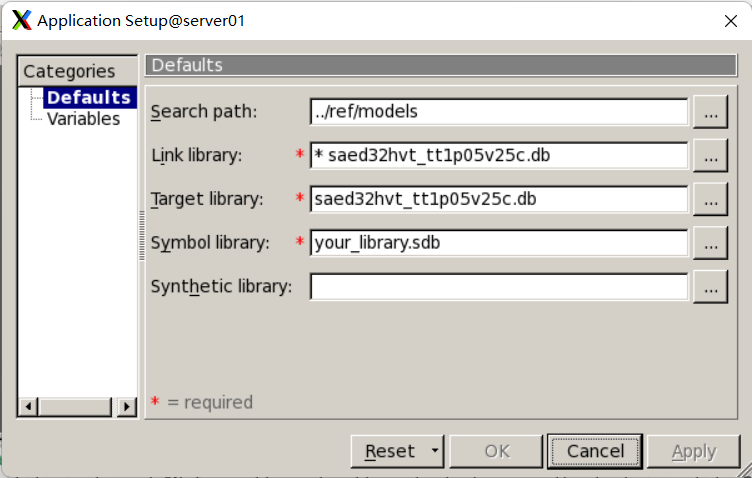
\includegraphics[width=0.7\textwidth]{images/4.png}
        \caption{Application setup window.}
    \end{figure}
    \begin{minted}{tcl}
source ../scripts/setup.tcl
    \end{minted}
    In IC Compiler, you specify the .db files to use for the design by setting target\_library and link\_library variables:
    \begin{itemize}
        \item The target\_library variable specifies the .db library files containing the logic cells that can be used for optimization, for example, different NAND gates having various areas, drive strengths, delays, and power usage.
        \item The link\_library variable specifies the .db libraries containing all the logic cells that can be used to resolve hierarchical references in the design during the execution of the link command.
    \end{itemize}
    \item Use the script created to carry out complex commands. There is \texttt{definitions.tcl} script in the \texttt{scripts} directory. To source the script, write:
    \begin{minted}{tcl}
source ../scripts/definitions.tcl
    \end{minted}
    Alternatively (and recommended the first time you run the flow), you can also run all steps of the definitions.tcl script manually as follows.
    \begin{enumerate}
        \item To create the Milkyway design library, Choose File > Create Library.
        \begin{figure}[H]
            \centering
            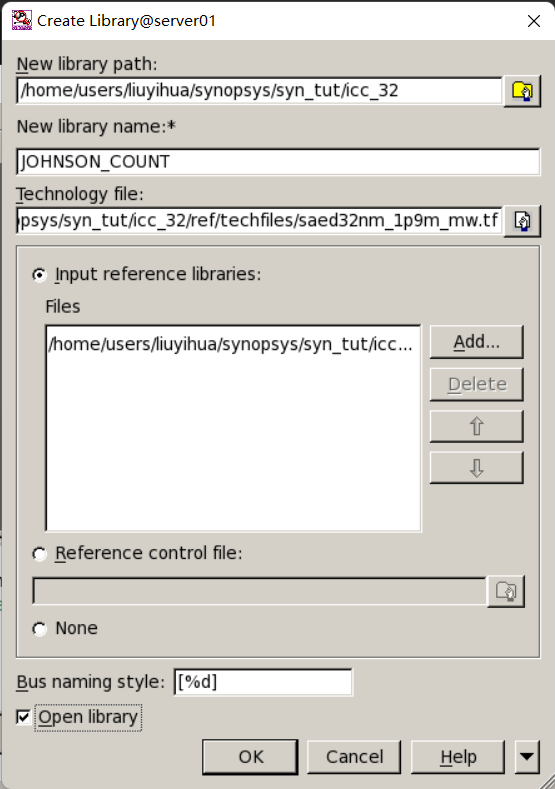
\includegraphics[width=0.55\textwidth]{images/5.png}
            \caption{Create library window.}
        \end{figure}
        The \texttt{create\_mw\_lib} command and the Create Library dialog box have options to specify the name of the new Milkyway library, the name of the associated technology file, the names of the associated Milkyway reference libraries, and the bus naming style. \textit{Remember to check "Open library". The warnings shown in the output can be ignored}:
        \begin{minted}[breaklines,breakanywhere]{text}
Start to load technology file /home/users/<username>/synopsys/syn_tut/icc_32/ref/techfiles/saed32nm_1p9m_mw.tf.
Warning: Layer 'M1' has a pitch 0.152 that does not match the recommended wire-to-via pitch 0.13 or 0.105. (TFCHK-049)
Warning: Layer 'M2' has a pitch 0.152 that does not match the recommended wire-to-via pitch 0.139. (TFCHK-049)
Warning: Layer 'M3' has a pitch 0.304 that does not match the recommended wire-to-via pitch 0.139. (TFCHK-049)
Warning: Layer 'M4' has a pitch 0.304 that does not match the recommended wire-to-via pitch 0.139. (TFCHK-049)
Warning: Layer 'M5' has a pitch 0.608 that does not match the recommended wire-to-via pitch 0.139. (TFCHK-049)
Warning: Layer 'M6' has a pitch 0.608 that does not match the recommended wire-to-via pitch 0.139. (TFCHK-049)
Warning: Layer 'M7' has a pitch 1.216 that does not match the recommended wire-to-via pitch 0.139. (TFCHK-049)
Warning: Layer 'M8' has a pitch 1.216 that does not match the recommended wire-to-via pitch 0.179 or 0.164. (TFCHK-049)
Warning: Layer 'M9' has a pitch 2.432 that does not match the recommended wire-to-via pitch 1.74. (TFCHK-049)
Warning: Layer 'MRDL' has a pitch 4.864 that does not match the recommended wire-to-via pitch 4.5. (TFCHK-049)
Warning: Layer 'MRDL' has a pitch 4.864 that does not match the doubled pitch 2.432 or tripled pitch 3.648. (TFCHK-050)
Warning: CapModel sections are missing. Capacitance models should be loaded with a TLU+ file later. (TFCHK-084)
Technology file /home/users/<username>/synopsys/syn_tut/icc_32/ref/techfiles/saed32nm_1p9m_mw.tf has been loaded successfully.
{JOHNSON_COUNT}
        \end{minted}
        \item TLUPlus is a binary table format that stores the RC coefficients. The TLUPlus models enable accurate RC extraction results by including the effects of width, space, density, and temperature on the resistance coefficients. Choose File > Set TLU+ (Figure \ref{f6}).
        \begin{figure}[H]
            \centering
            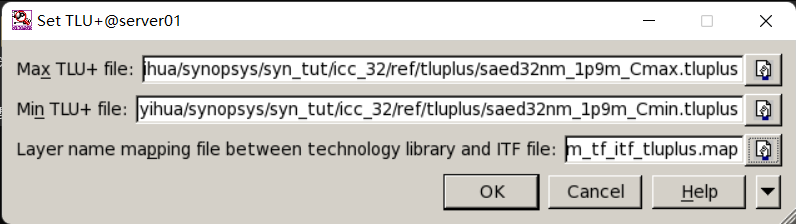
\includegraphics[width=\textwidth]{images/6.png}
            \caption{Set TLU+ window.}
            \label{f6}
        \end{figure}
        Type or browse for the map file in the “Map file” text box. Type or browse for the maximum and minimum TLUPlus model files.
        \item Import Design - Read the Verilog file for the design by choosing File > Import > Read Verilog... and specifying the Verilog netlist file, which is a gate-level design in one or more files (Figure \ref{f7} and Figure \ref{f8}).
        \begin{figure}[H]
            \centering
            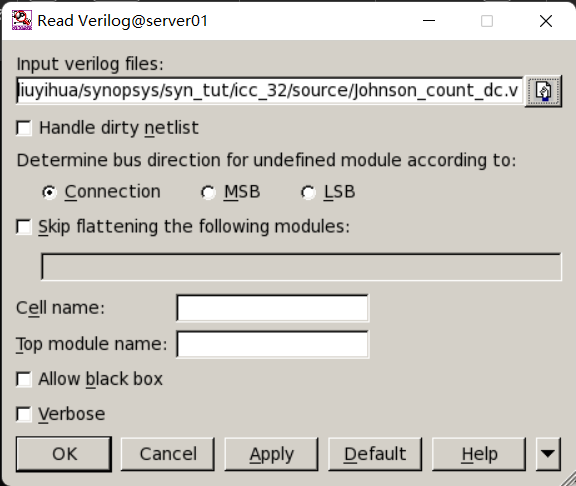
\includegraphics[width=\textwidth]{images/7.png}
            \caption{Import design window.}
            \label{f7}
        \end{figure}
        If \texttt{import\_designs} failed with errors, please go to Appendix \ref{AImp}. The Cell name and the Top module name can be left empty as IC Compiler will automatically specify them from the Input Verilog files.
        \begin{figure}[H]
            \centering
            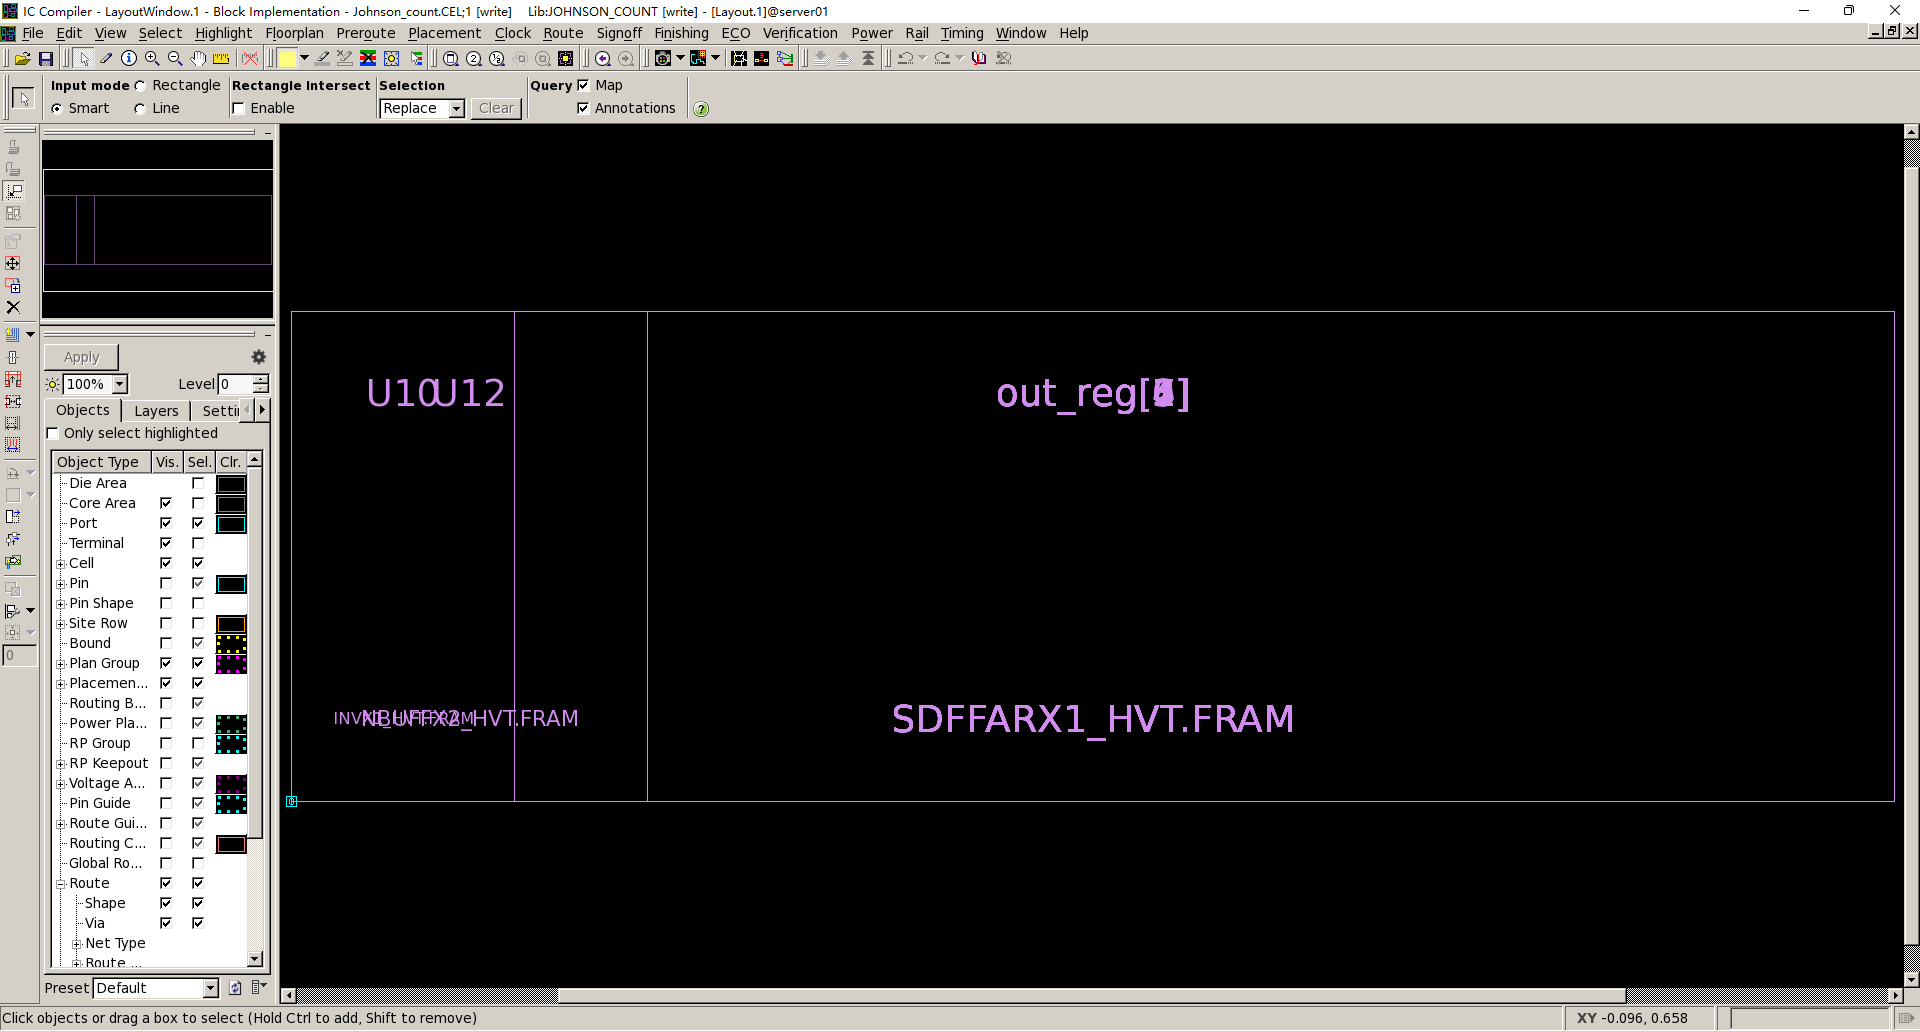
\includegraphics[width=\textwidth]{images/8.png}
            \caption{Design view after importing.}
            \label{f8}
        \end{figure}
        \item To source constraints with .sdc (Synopsys Design Constraints) format:
        \begin{minted}{text}
icc_shell> source ../source/constr.sdc
        \end{minted}
    \end{enumerate}
    \item Use script created to carry out complex commands. There is a script in \texttt{scripts} directory. The name of this script: \texttt{design\_all.tcl}. To source the script, write:
    \begin{minted}{text}
icc_shell> source ../scripts/design_all.tcl
    \end{minted}
    Now show the steps of \texttt{design\_all.tcl} script. Note that commands in the script and following steps with GUI are not identical, even though they yield similar layouts.
    \begin{itemize}
        \item Initialize floorplan; declare power nets and pins
        \item Create rectangular rings
        \item Create power straps
        \item Core Placement and Optimization
        \item Core CTS (Clock Tree synthesis) and Optimization 
        \item Preroute standard cells
        \item Core Routing and Optimization
        \item Inserting Fillers
    \end{itemize}
    \begin{enumerate}
        \item Floorplan information includes the core area, top-level ports, and placement sites.\\
        For floorplanning the design choose Floorplan->Create Floorplan... (Figure \ref{f9} and Figure \ref{f10}).
        \begin{figure}[H]
            \centering
            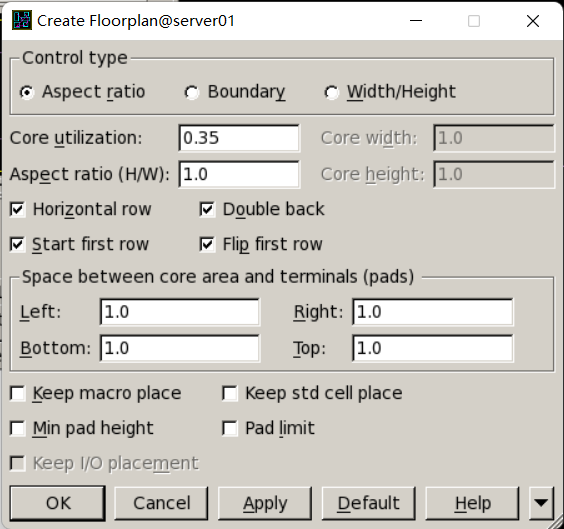
\includegraphics[width=0.8\textwidth]{images/9.png}
            \caption{Initialize floorplan window.}
            \label{f9}
        \end{figure}
        Specify the control parameters.\\
        Indicate the method which specifies the size of the core area:
        \begin{enumerate}
            \item Aspect ratio – A ratio of height divided by width (the default)
            \item Width \& height – The exact width and height
            \item Row number – A number of rows
            \item Boundary – A fixed size according to the boundary defined in design planning
        \end{enumerate}
        \textit{If the design view does not show the name labels, it is because the name labeling is set to "Both" by default, and there is not enough space to show both the instance name and the reference name. You can zoom in the design view to see the full labels. To only show the instance name, go to the "Settings" tab->"Cells" tab, and in the "Name labeling" frame, select "Instance name". You can save the design and reopen it by}
        \begin{minted}[breaklines]{tcl}
open_mw_lib /home/users/<username>/synopsys/syn_tut/icc_32/JOHNSON_COUNT
::iccGUI::open_mw_cel  Johnson_count
open_mw_cel Johnson_count
        \end{minted}
        \textit{If you failed to open the design with error}
        \begin{minted}[breaklines]{text}
open_mw_cel Johnson_count
INFO: cell is locked by <username> (pid 446498 server01) check again...
INFO: cell is locked by <username> (pid 446498 server01) check again...
INFO: cell is locked by <username> (pid 446498 server01) check again...
INFO: cell is locked by <username> (pid 446498 server01) check again...
INFO: cell is locked by <username> (pid 446498 server01) check again...
INFO: Could not lock the cell for write, giving up
INFO: Please remove the lock to proceed.
Error: Failed to open design:'Johnson_count.CEL;0'for 'w'. (MWUI-007)
        \end{minted}
        \textit{Please remove \texttt{/home/users/<username>/synopsys/syn\_tut/icc\_32/JOHNSON\_\\
        COUNT/CEL/Johnson\_count:1.lock} file}.
        \begin{figure}[H]
            \centering
            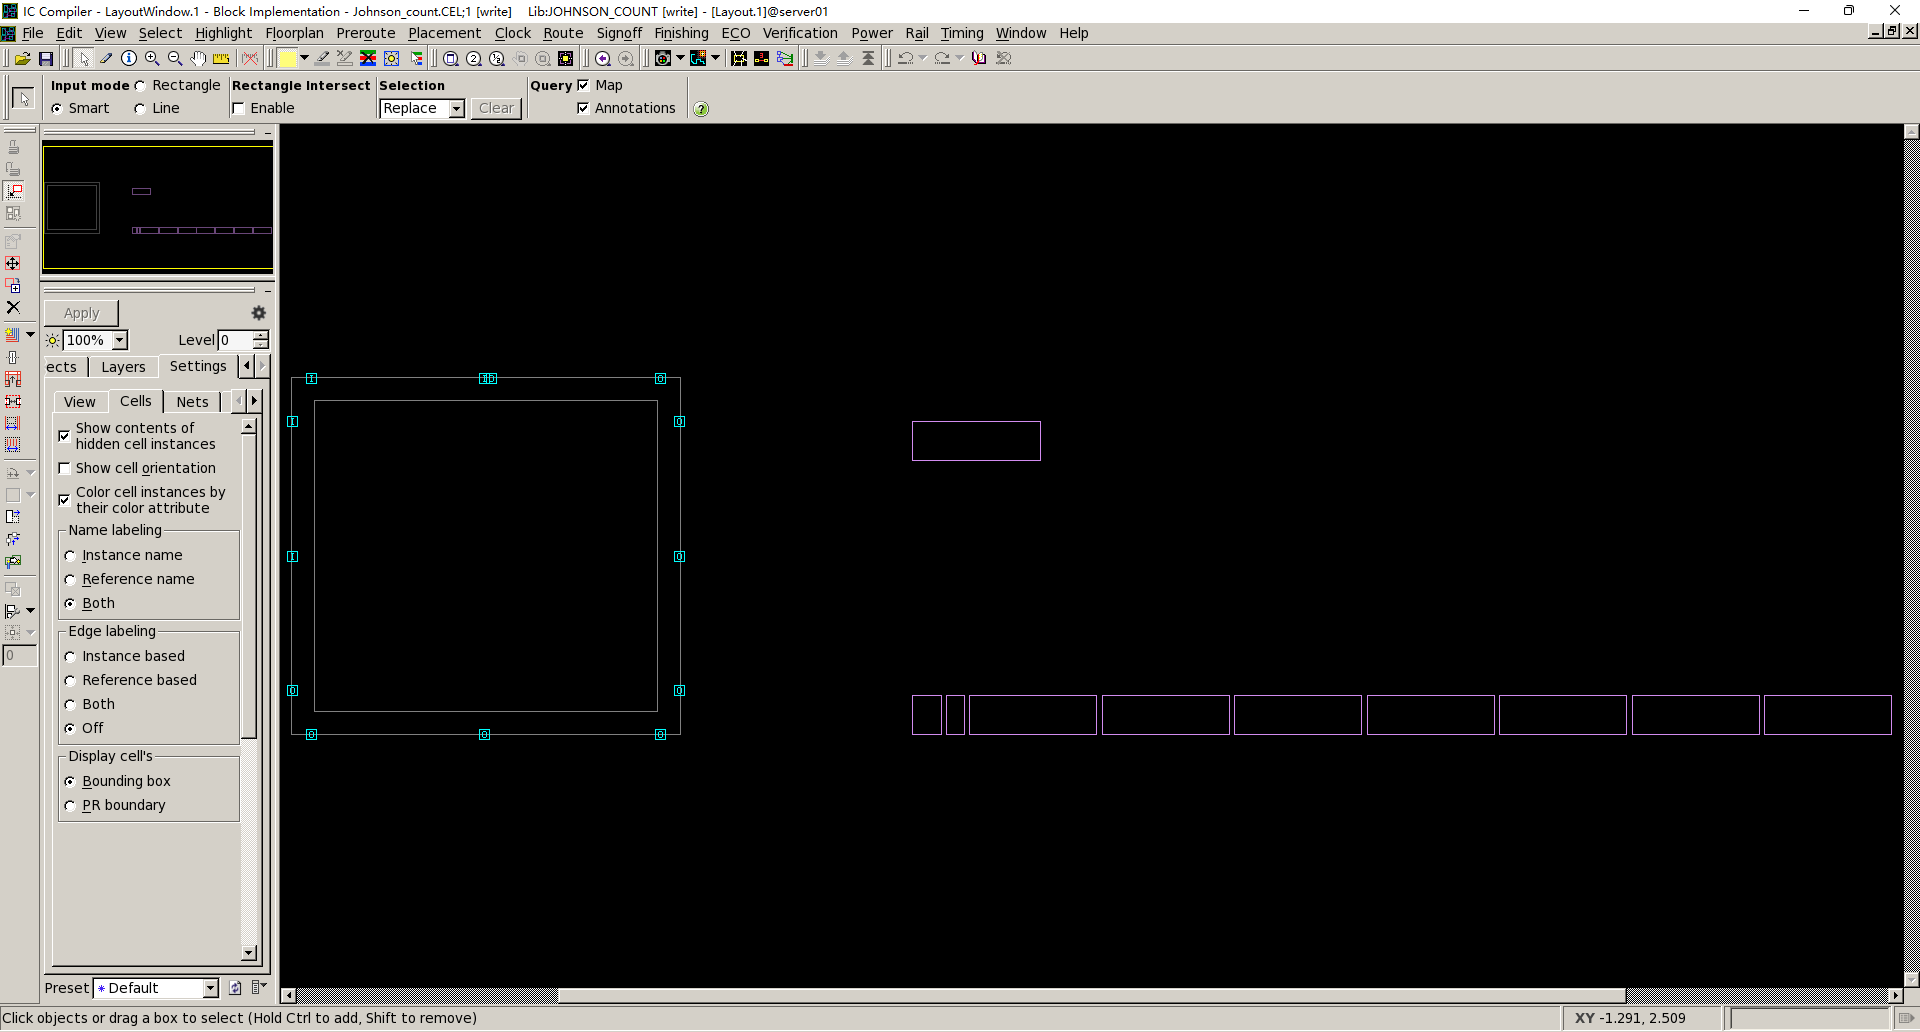
\includegraphics[width=\textwidth]{images/10.png}
            \caption{Design view after \texttt{initialize\_floorplanning}.}
            \label{f10}
        \end{figure}
        Declare power nets and pins.\\
        Type into the ICC shell the following:
        \begin{minted}[breaklines]{tcl}
set power "VDD"
set ground "VSS"
set powerPort "VDD"
set groundPort "VSS"
set mw_logic0_net "VSS"
set mw_logic1_net "VDD"
derive_pg_connection -power_net VDD -ground_net VSS -power_pin VDD -ground_pin VSS
        \end{minted}
        \item Add power and ground rings.\\
        To add power and ground rings, choose PreRoute > Create Rings. Select the Rectangular tab (Figure \ref{f11} and Figure \ref{f12})
        \begin{figure}[H]
            \centering
            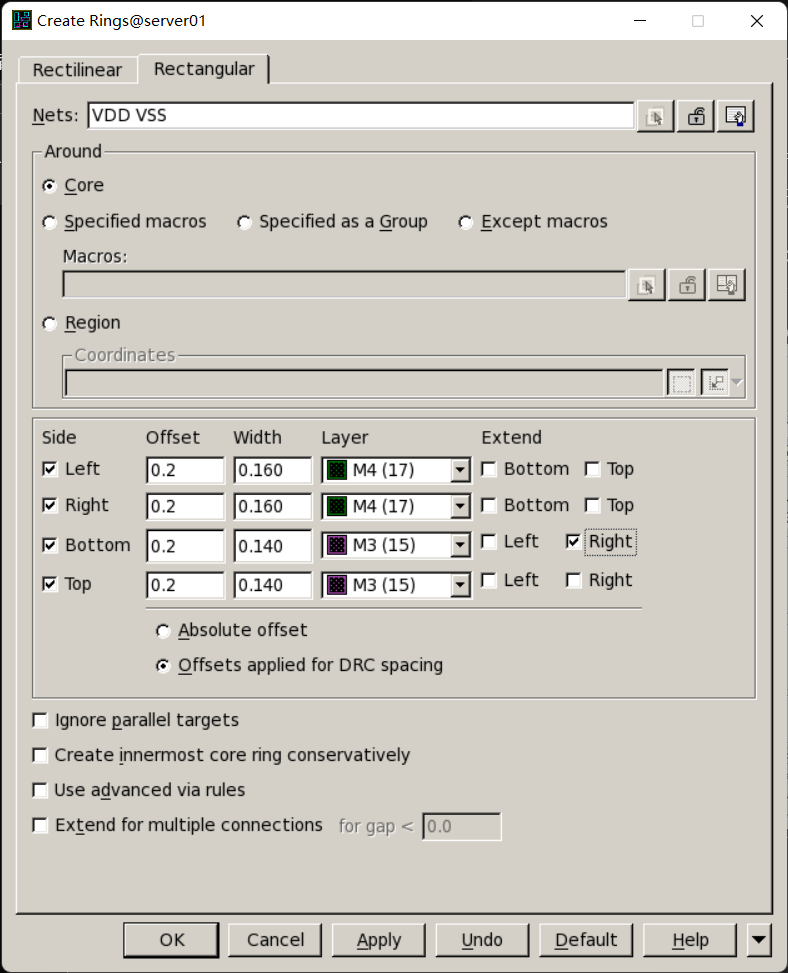
\includegraphics[width=0.75\textwidth]{images/11.png}
            \caption{Create rectangular rings window.}
            \label{f11}
        \end{figure}
        \begin{figure}[H]
            \centering
            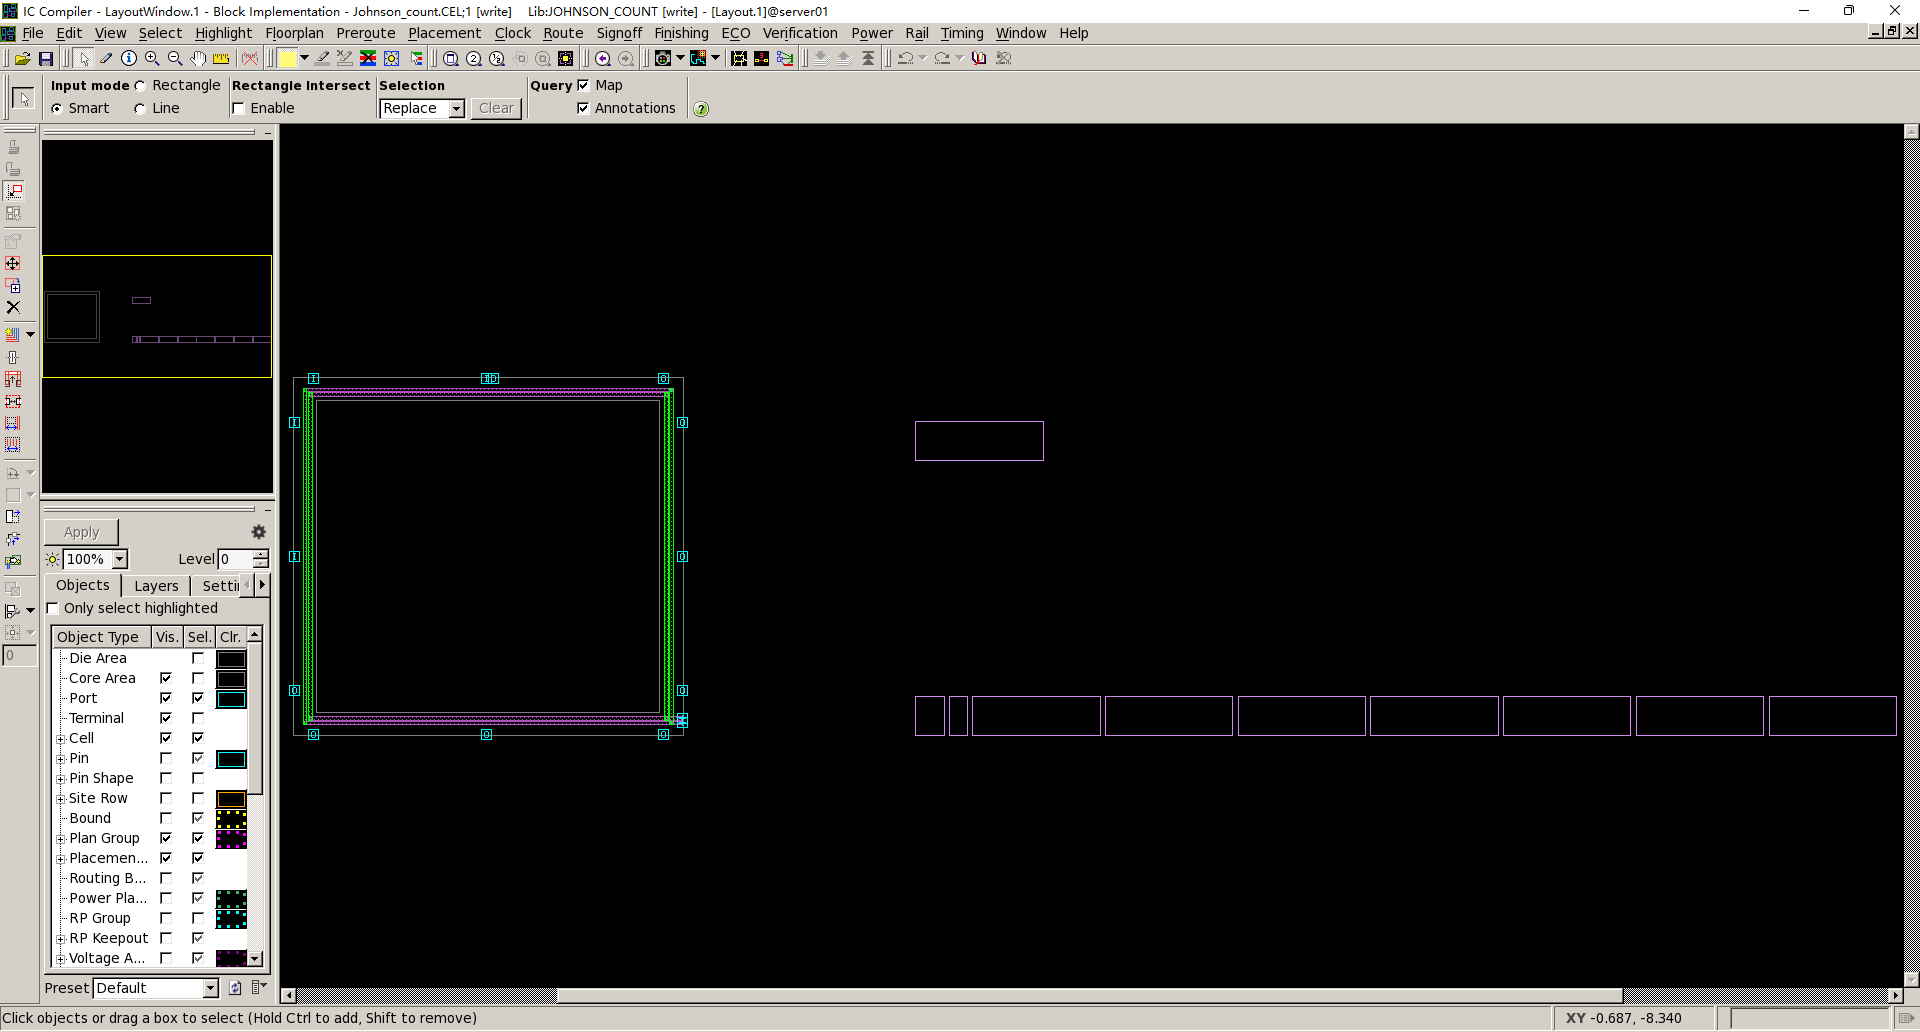
\includegraphics[width=\textwidth]{images/12.png}
            \caption{Design view after the creation of rectangular rings.}
            \label{f12}
        \end{figure}
        \item After the creation of rectangular rings, the straps are automatically connected to the closest power and ground ring at, or beyond, both ends of the straps.
        \begin{figure}[H]
            \centering
            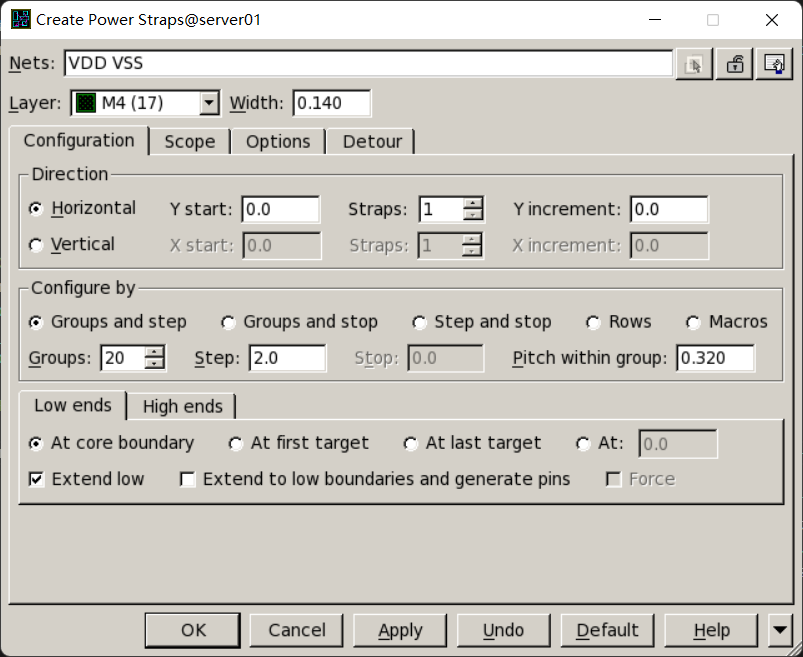
\includegraphics[width=0.8\textwidth]{images/13.png}
            \caption{Create object tool window.}
            \label{f13}
        \end{figure}
        The \texttt{create\_power\_straps} command creates power straps in a design. Use a few wide straps rather than many thin straps to improve the placement quality and decrease the placement runtime.\\
        The same as from the Menu bar, choose PreRoute > Create Power Straps... (Figure \ref{f13} and Figure \ref{f14}).\\
        Choose vertical and horizontal metal layers accordingly, and do vertical and horizontal power straps separately.
        % \textbf{Take a screenshot of your Design view after creating power straps}.
        \begin{figure}[H]
            \centering
            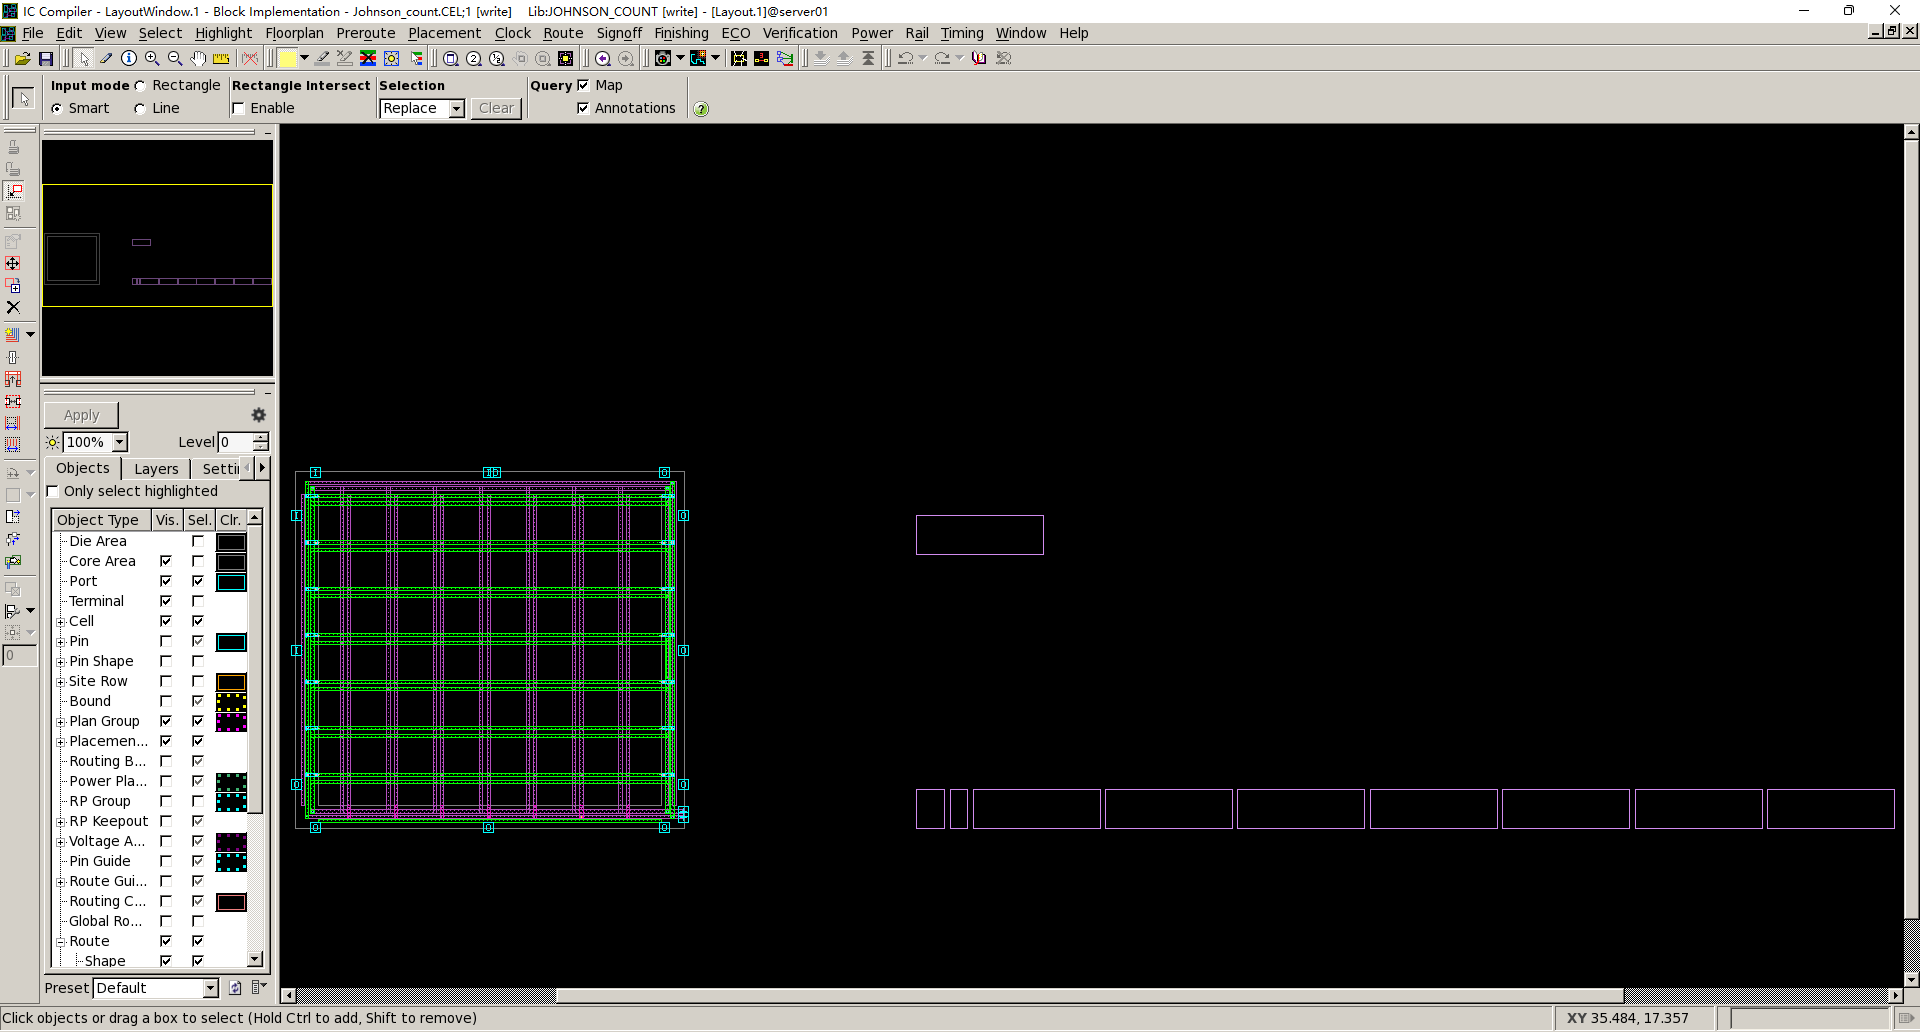
\includegraphics[width=\textwidth]{images/14.png}
            \caption{Design view after creation power straps.}
            \label{f14}
        \end{figure}
        \textit{You need to choose the core utilization, groups, and the step in a proper range in order to fit the floorplan. Please show your choice}.
        \item \texttt{place\_opt} command performs simulation placement, routing, and optimization on the current design. During the placement phase, this design's standard cells have been automatically placed in horizontal placement rows.
        \begin{figure}[H]
            \centering
            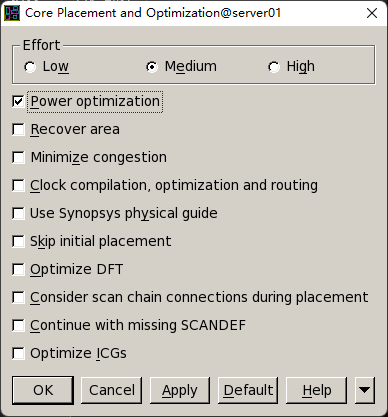
\includegraphics[width=0.6\textwidth]{images/15.png}
            \caption{Core placement and optimization window.}
            \label{f15}
        \end{figure}
        To run placement, choose Placement > Core Placement and Optimization... (Figure \ref{f15} and Figure \ref{f17})
        \begin{figure}[H]
            \centering
            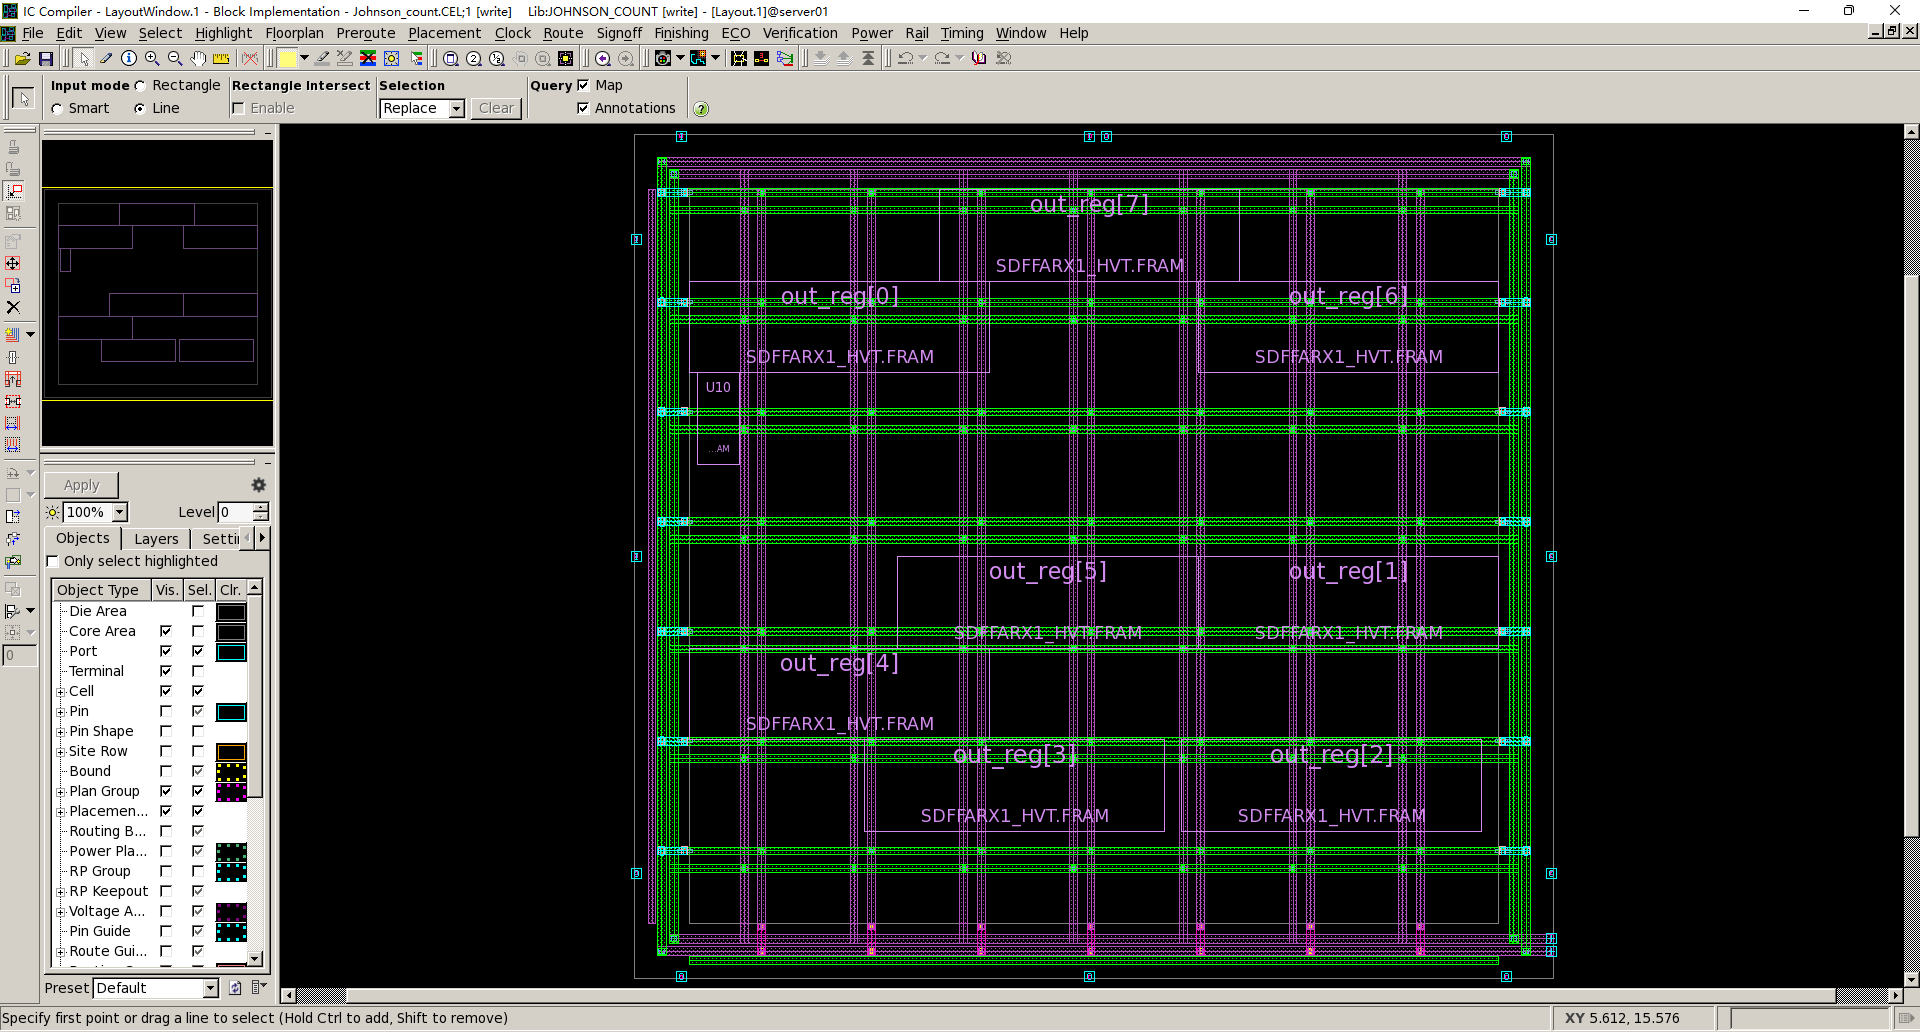
\includegraphics[width=\textwidth]{images/17.png}
            \caption{Design view after Core Placement and Optimization.}
            \label{f17}
        \end{figure}
        The "Core Placement and Optimization@server01" dialog box appears. Select “Power optimization”. \textit{The effort can be medium or high; also select "Optimize DFT" or "Continue with missing SCANDEF", and optionally "Minimize congestion"; otherwise, you will fail with errors}:
        \begin{minted}[breaklines]{text}
Error: Initial placement includes scan chains but no scan DEF information. Aborting. Issue "man PSYN-1072" for information on avoiding this. (PSYN-1072)
        \end{minted}
        \begin{figure}[H]
            \centering
            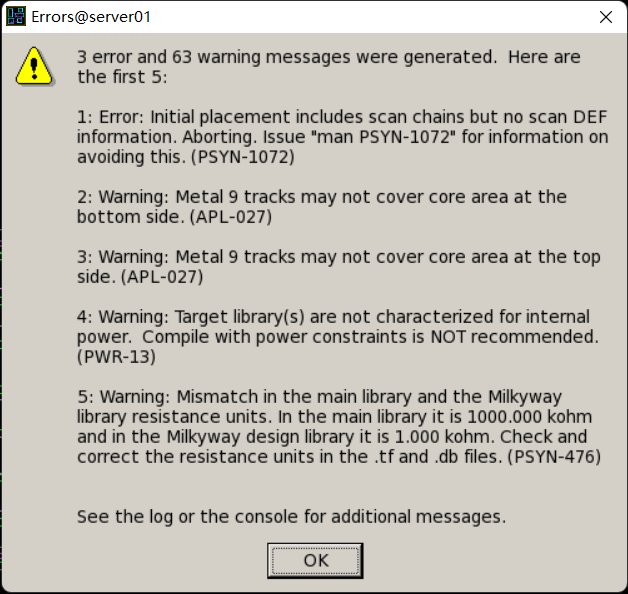
\includegraphics[width=\textwidth]{images/16.png}
        \end{figure}
        \textit{The documentation can be accessed by \texttt{man PSYN-1072}. Or you can also start from the Placement menu->Coarse Placement... and also check the necessary options of configuration. Selecting the effort to high produces less density. If the density is too high, it will fail with errors}:
        \begin{minted}[breaklines]{text}
Warning: Density is 99.9% (PSYN-1010)
Initial legalization:  10% 20% 30% 40% 50% 60% 70% 80% 90% 100% (0 sec)
Error: Could not find a legal placement.
Legalization complete (0 total sec)
Top 5 lib cells with lowest legal rate;
Error: A legal placement could not be found (PSYN-044)
        \end{minted}
        and
        \begin{minted}[breaklines]{text}
Warning: Metal 9 tracks may not cover core area at the bottom side (APL-027)
Warning: Metal 9 tracks may not cover core area at the top side (APL-027)
Error: An error has occurred in the execution of the detailed placer. (PSYN-060)

  Placement Optimization complete
  -------------------------------

Error: psynopt has abnormally terminated.  (OPT-100)
Warning: ICC has suggestions for improving your design.  Use "report_suggestions" for details.  (PSYN-1067)
        \end{minted}
        \item Clock tree synthesis. During clock tree synthesis, IC Compiler builds clock trees that meet the clock tree design rule constraints while balancing the loads and minimizing the clock skew. IC Compiler fixes the placement of the clock sinks, performs incremental logic and placement optimization, and fixes the placement of both the buffers and registers on the clock tree. The \texttt{clock\_opt} command performs clock tree synthesis, routing of clock nets, extraction, optimization, and optionally hold-time violation fixing on the current design. If clock tree synthesis fails or the routing of clock nets fails, the command returns a value of 0.
        \begin{figure}[H]
            \centering
            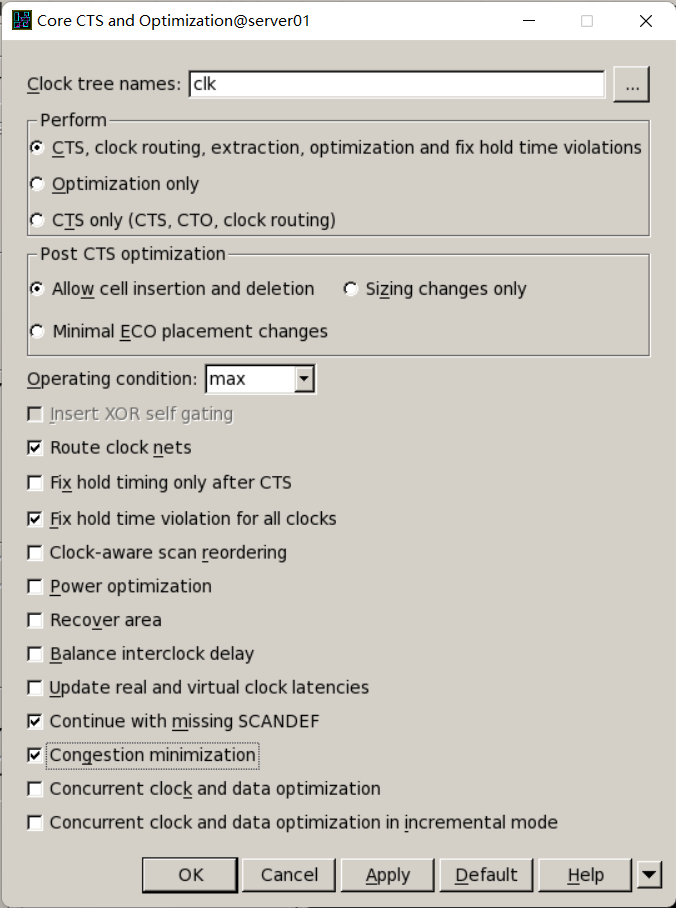
\includegraphics[width=\textwidth]{images/18.png}
            \caption{Core CTS and optimization window.}
            \label{f18}
        \end{figure}
        To perform clock tree synthesis and optimization, use the \texttt{clock\_opt} command or choose Clock > Core CTS and Optimization... in the GUI (Figure \ref{f18} and Figure \ref{f20}).\\
        The "Core CTS and Optimization@server01" dialog box appears, and select route clock cells. \textit{In the Perform frame, you can select "CTS, clock routing, extraction, optimization and fix hold time violations" or "Optimize only" or previously "Incremental optimization only (clock routing, extraction, optimization, and fix hold time)". You can also optionally check "Congestion minimization" and "Fix hold time violation for all clocks". Also, remember to check "Continue with missing SCANDEF"; otherwise, it will fail with errors}:
        \begin{minted}[breaklines]{text}
Error: Placement includes scan chains but no scan DEF information. Aborting. Issue "man PSYN-1096" for information on avoiding this. (PSYN-1096)
        \end{minted}
        \begin{figure}[H]
            \centering
            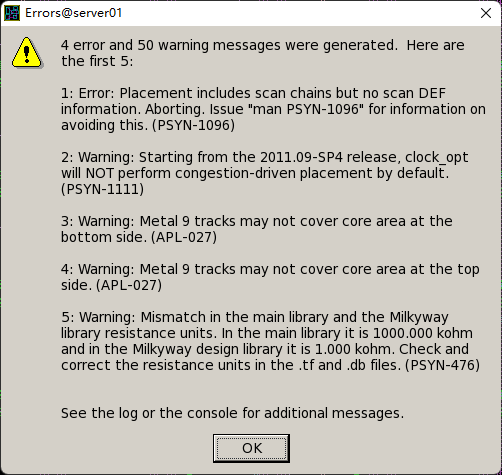
\includegraphics[width=\textwidth]{images/19.png}
        \end{figure}
        \textit{You need to make your own choices to produce a valid design}.
        \begin{figure}[H]
            \centering
            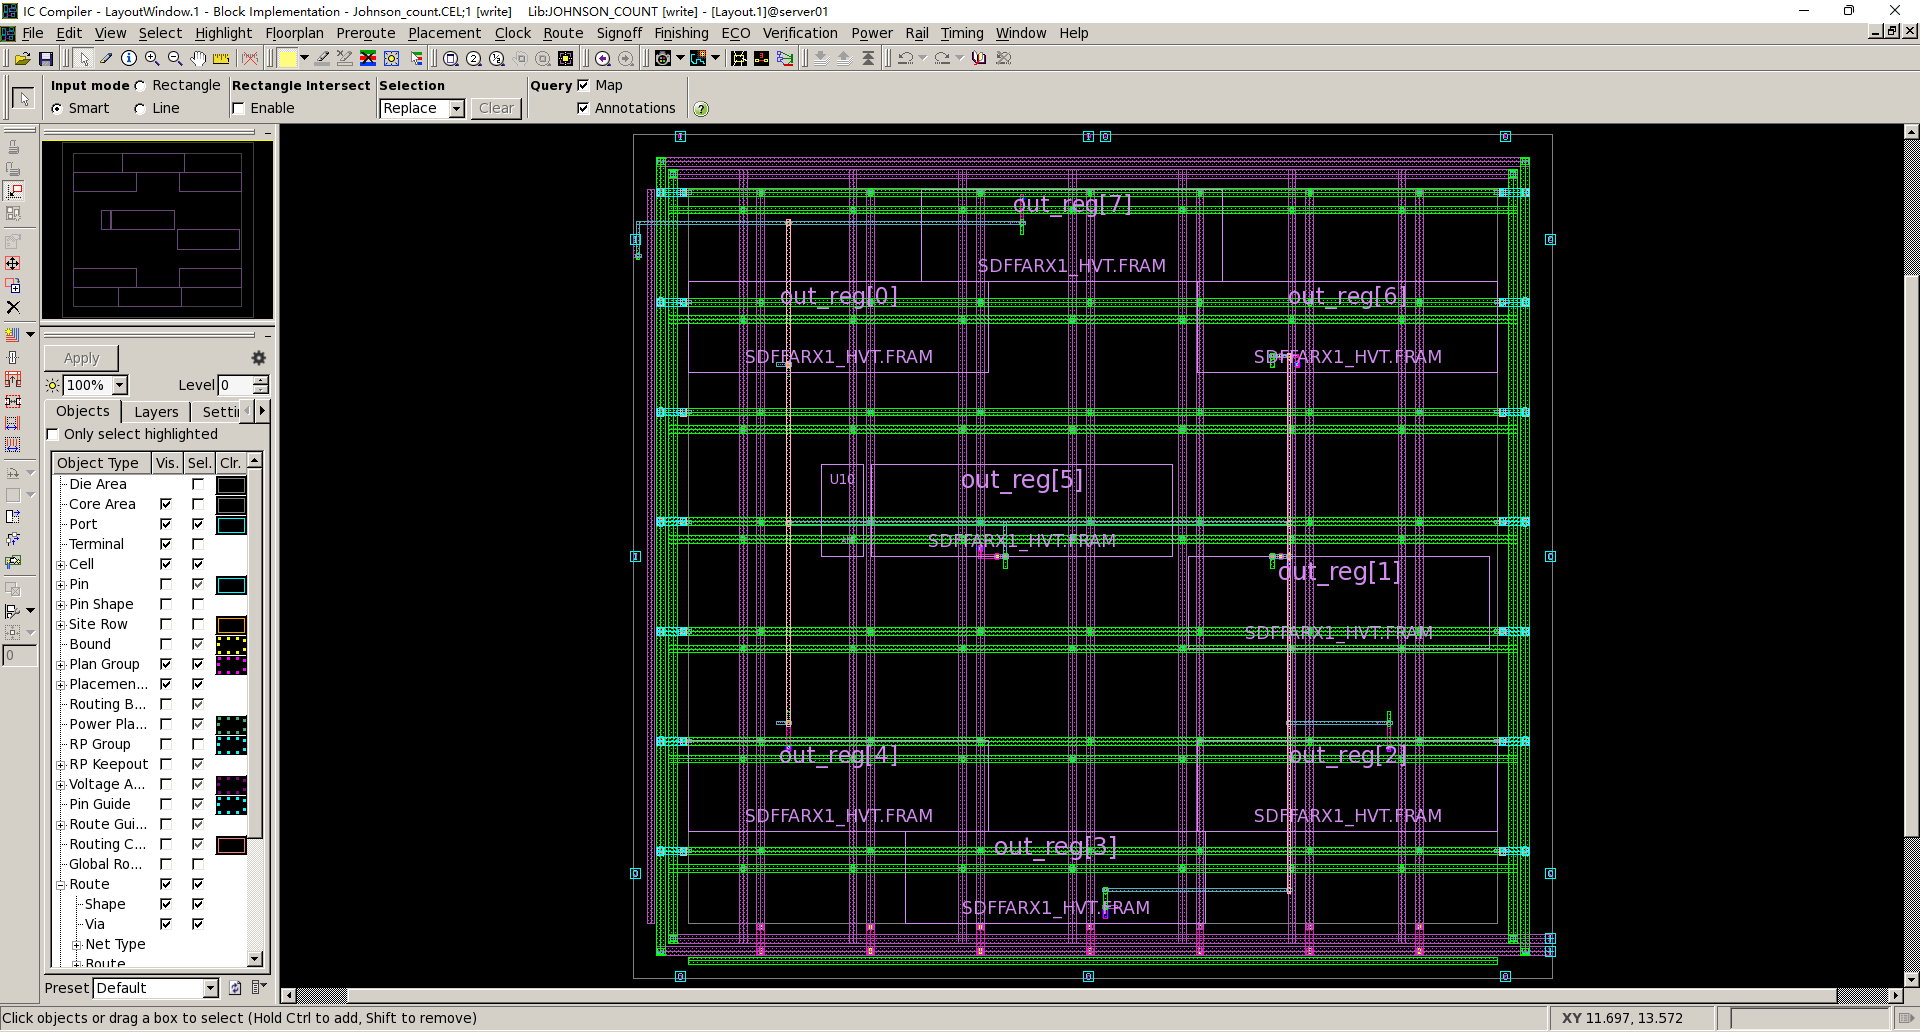
\includegraphics[width=0.9\textwidth]{images/20.png}
            \caption{Design view after Core CTS and Optimization.}
            \label{f20}
        \end{figure}
        \item Connect power and ground pins in standard cells to the straps and rings and connect power and ground rails in the standard cells. To make sure the global router can recognize the routing obstruction, preroute the standard cells before performing global routing.\\
        The \texttt{preroute\_standard\_cells} command connects power and ground pins in the standard cells to the power and ground rings or straps and connects power and ground rails in the standard cells.
        \begin{figure}[H]
            \centering
            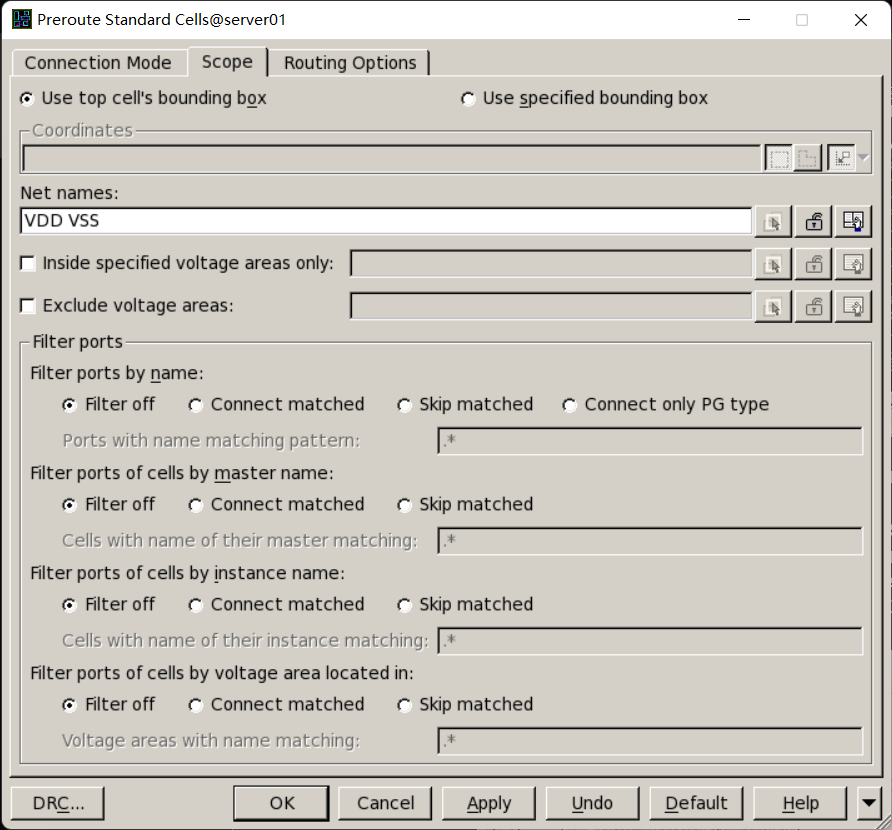
\includegraphics[width=0.6\textwidth]{images/21.png}
            \caption{Preroute standard cells window.}
            \label{f21}
        \end{figure}
        The same as from the Menu bar, choose PreRoute > Preroute Standard Cells... (Figure \ref{f21} and Figure \ref{f22}).
        \begin{figure}[H]
            \centering
            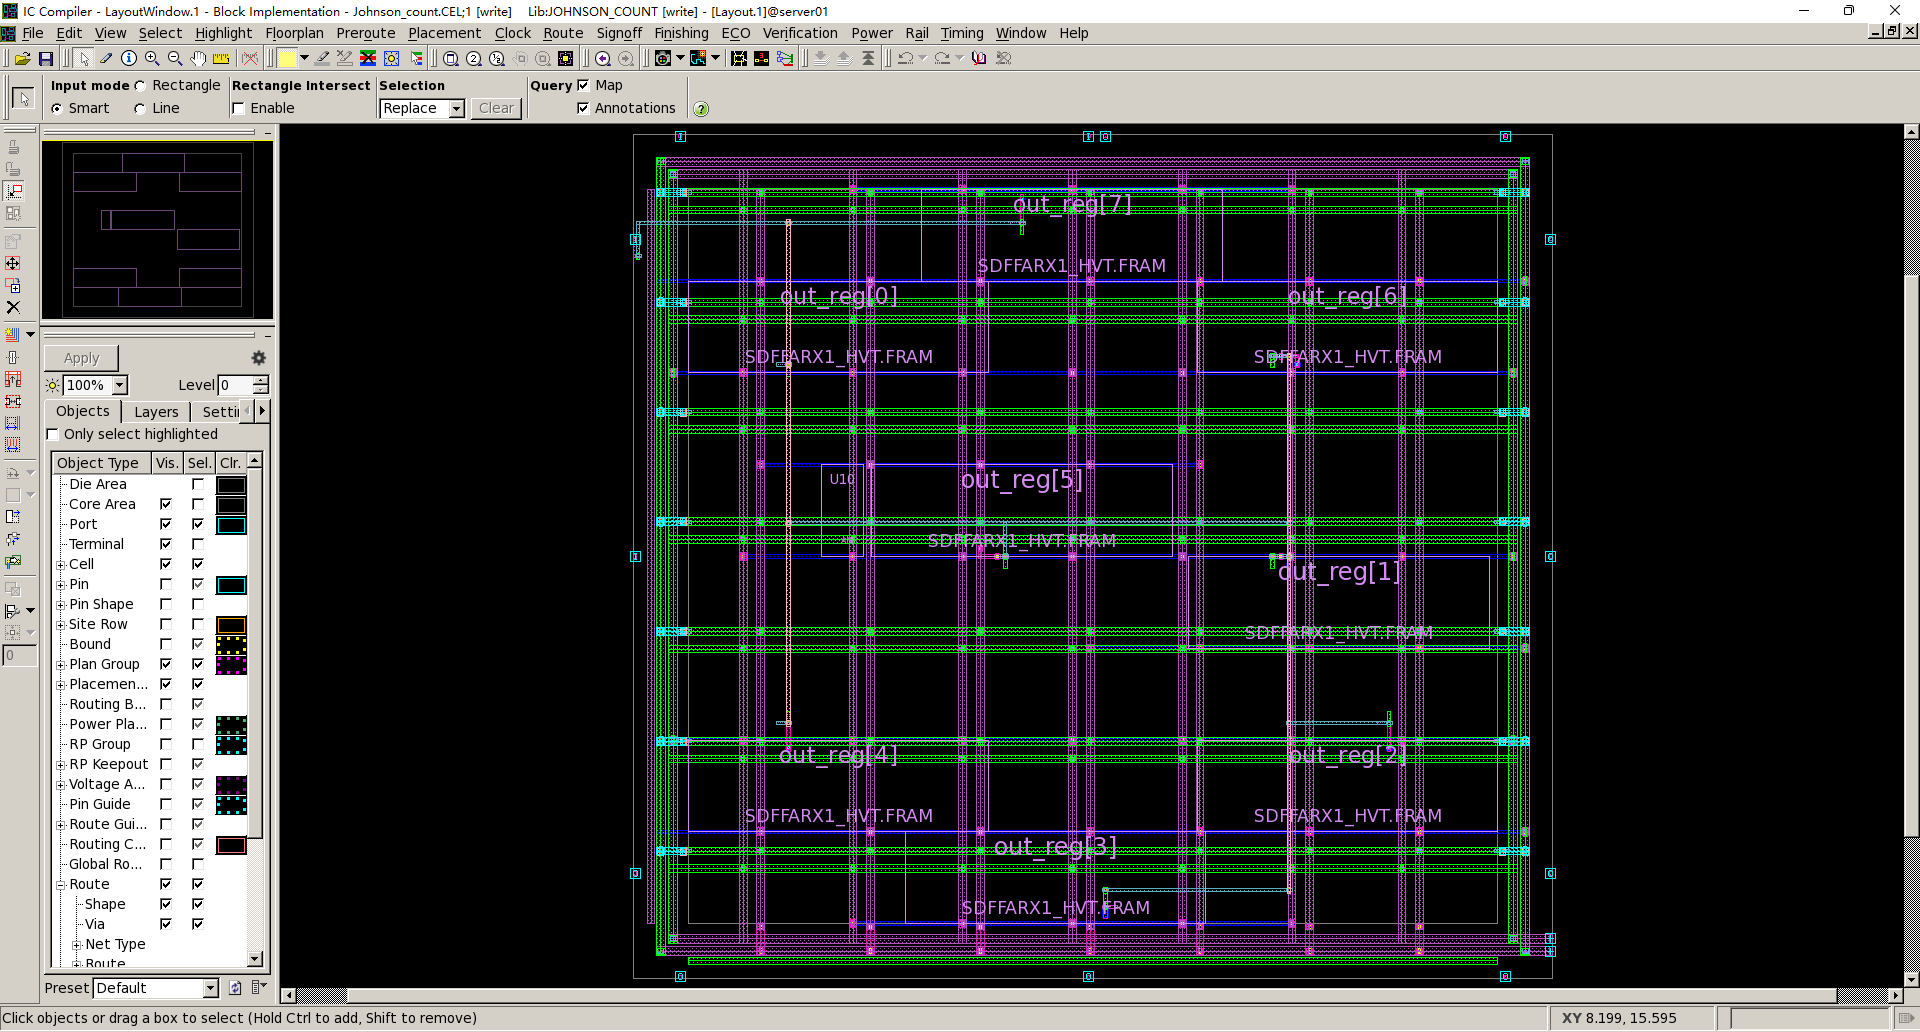
\includegraphics[width=0.8\textwidth]{images/22.png}
            \caption{Design view after Prerouting Standard Cells.}
            \label{f22}
        \end{figure}
        \item The \texttt{route\_opt} this command performs simultaneous routing and postroute optimization on the current design. The output of this command is a postroute-optimized design.
        \begin{figure}[H]
            \centering
            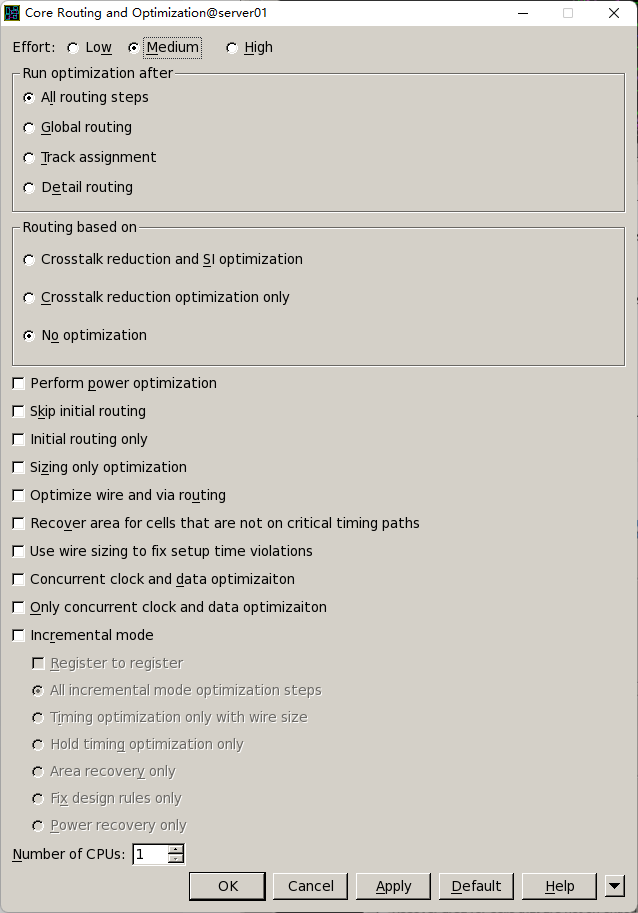
\includegraphics[width=0.45\textwidth]{images/23.png}
            \caption{Core routing and optimization window.}
            \label{f23}
        \end{figure}
        Finally, for routing the design, choose Route->Core Routing and Optimization. The "core routing and optimization" dialog box appears (Figure \ref{f23} and Figure \ref{f24}).
        \begin{figure}[H]
            \centering
            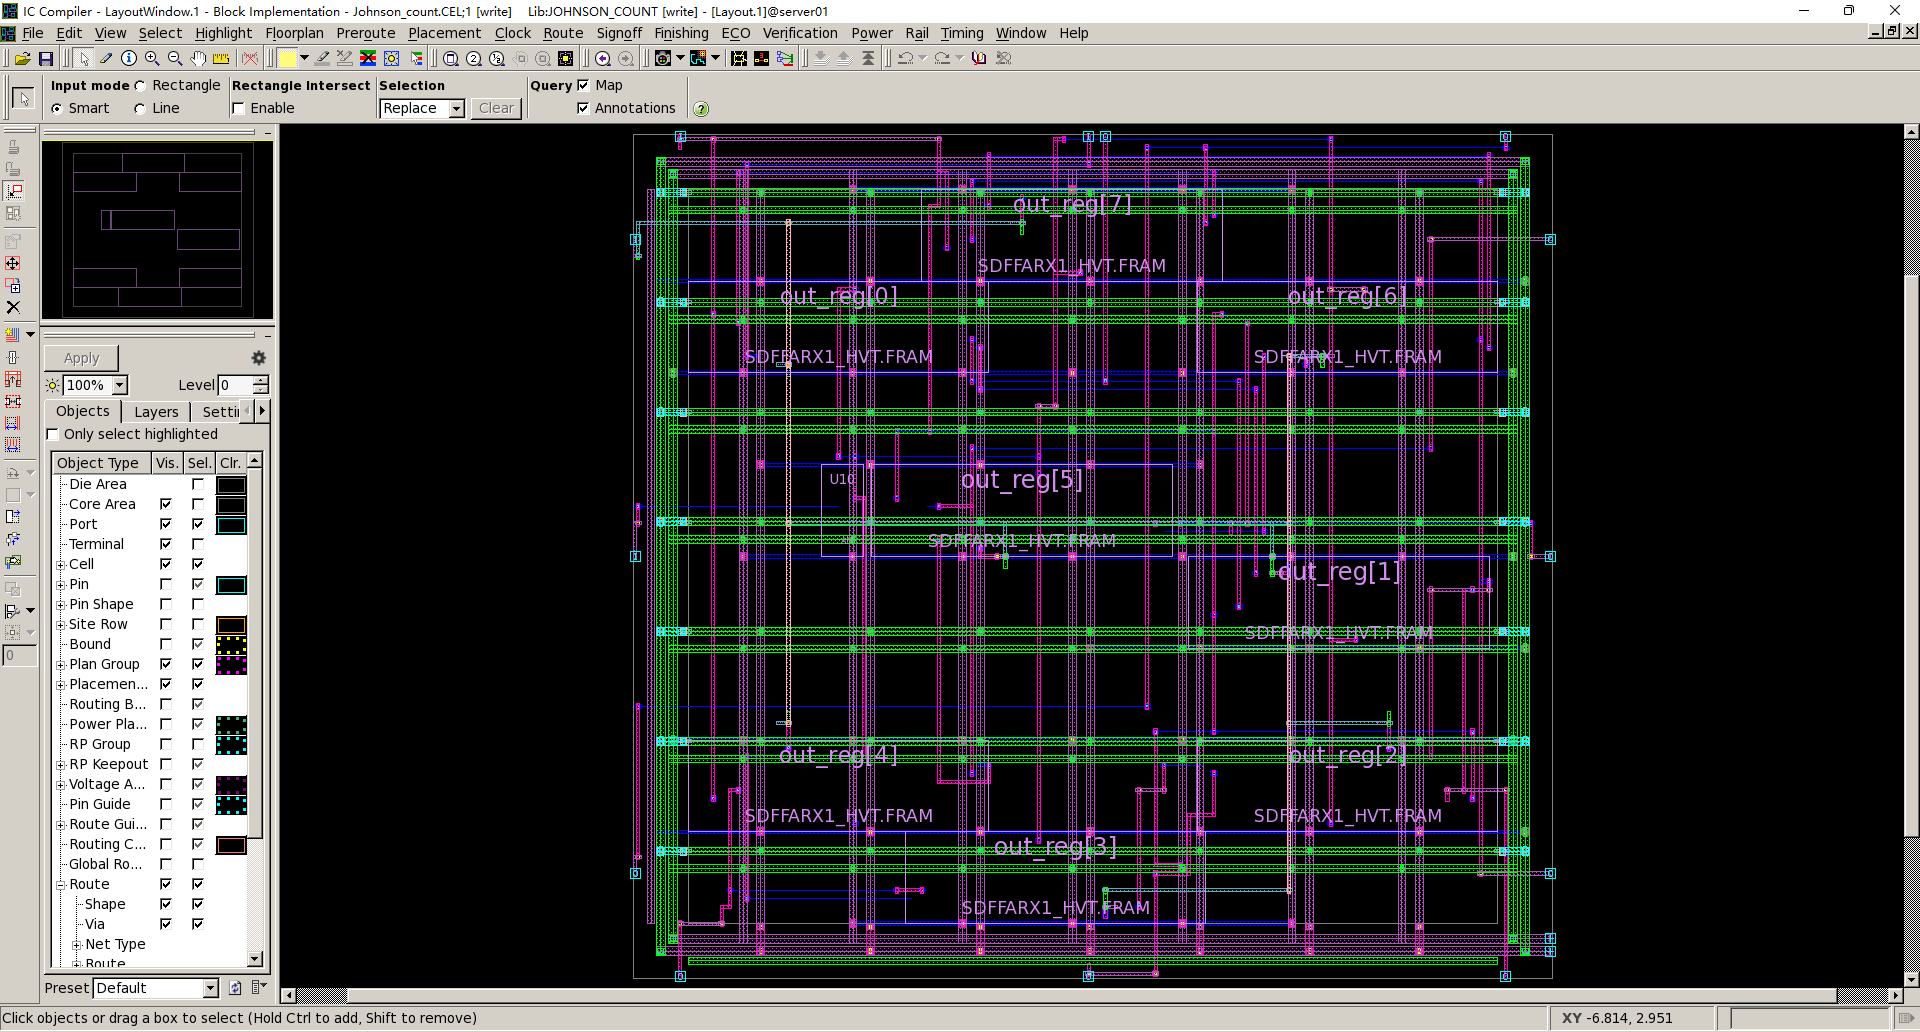
\includegraphics[width=\textwidth]{images/24.png}
            \caption{Design view after core routing and optimization.}
            \label{f24}
        \end{figure}
        ICC has \texttt{route\_eco} command. This command performs routing for the broken nets. It runs the global route, track assignment, and detail route.
        \item \texttt{insert\_stdcell\_filler} this command fills empty spaces in standard cell rows with instances of master filler cells in the library (Figure \ref{f25}).
        \begin{figure}[H]
            \centering
            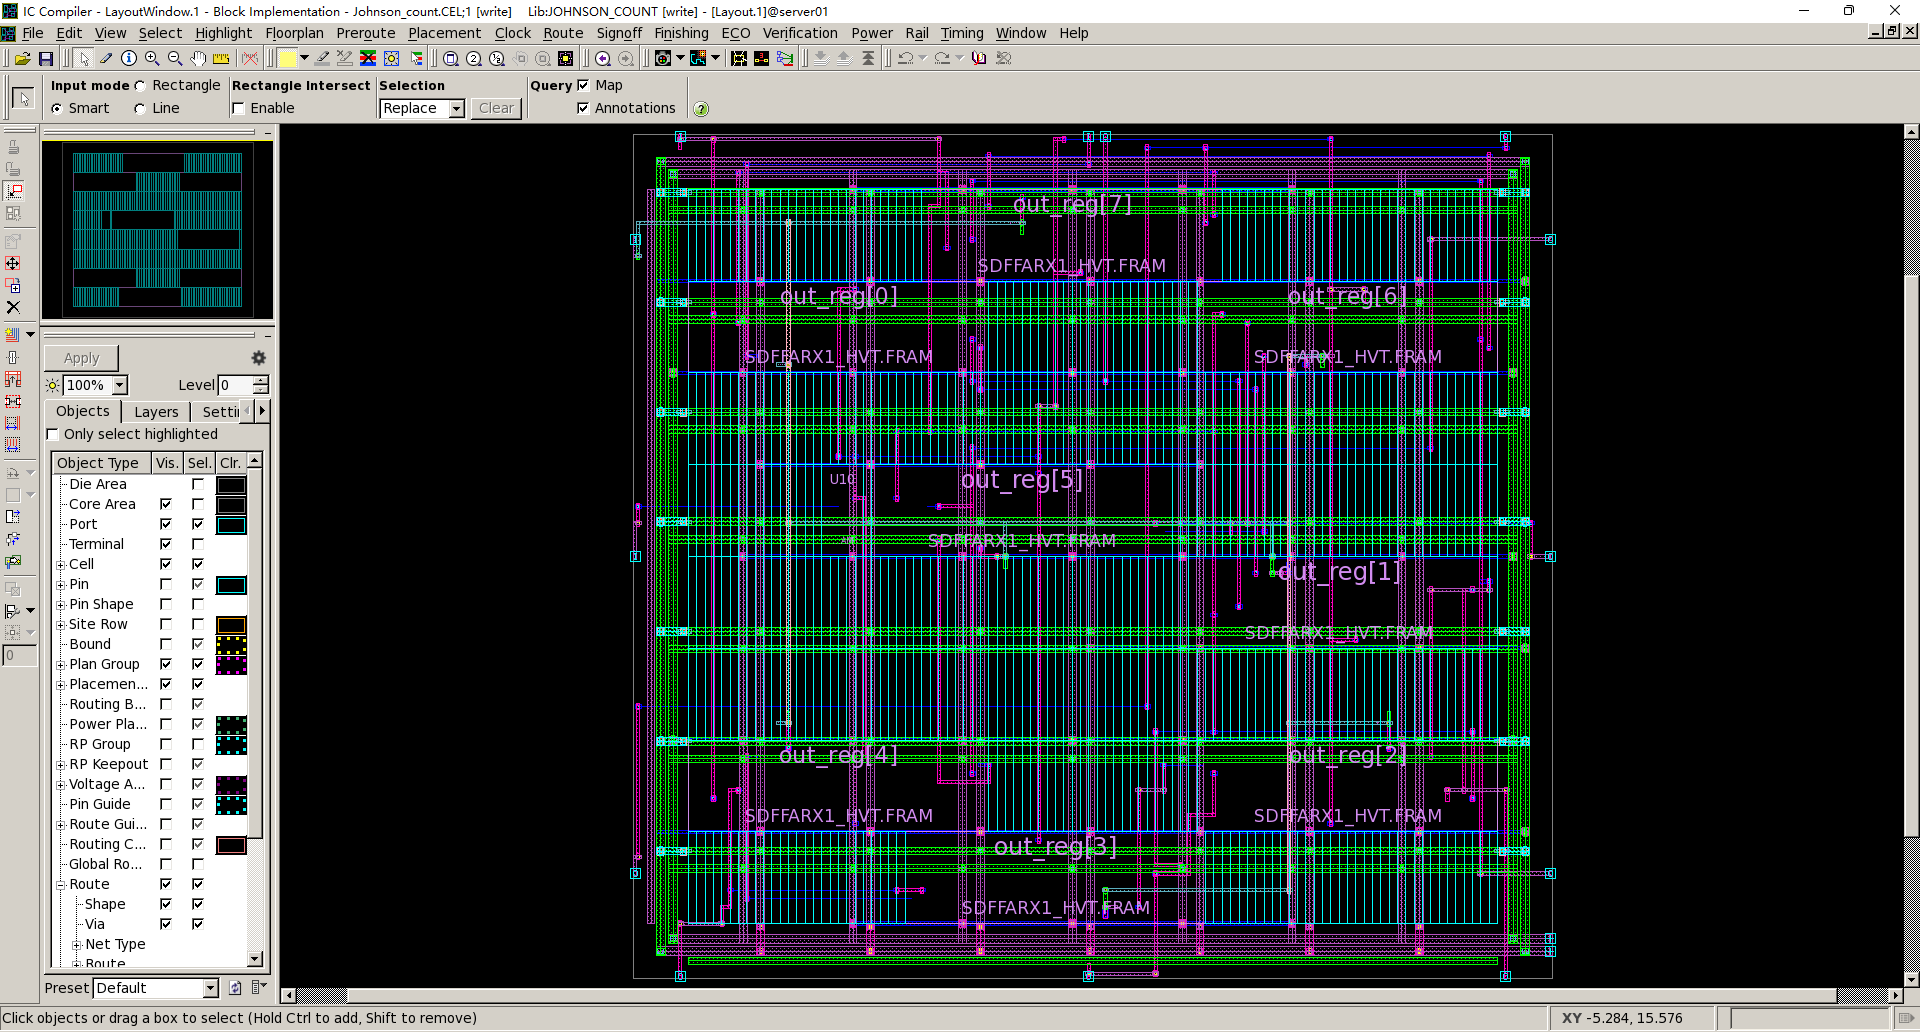
\includegraphics[width=0.9\textwidth]{images/25.png}
            \caption{Design view after insert fillers.}
            \label{f25}
        \end{figure}
        \textit{Make sure you are inserting correct stdcell filters as for your library. If not, you may get errors}:
        \begin{minted}[breaklines]{text}
Error: Nothing matched for collection (SEL-005)
ignorePGRail 1 ignoreDpt 1 ignoreBetweenFillers 1
User specify 0 filler masters
        \end{minted}
    \end{enumerate}
    \item IC Compiler allows checking DRC (Design Rule Checking) and LVS (layout-versus-schematic). To check DRC errors, choose Verification > Signoff DRC... \textit{The DRC requires Synopsys IC Validator (\texttt{icv}), which is, however, not set up on the server; thus, we have to skip this step; instead, we should run \texttt{extract\_rc} to extract the design and derive parasitics}.
    \begin{figure}[H]
        \centering
        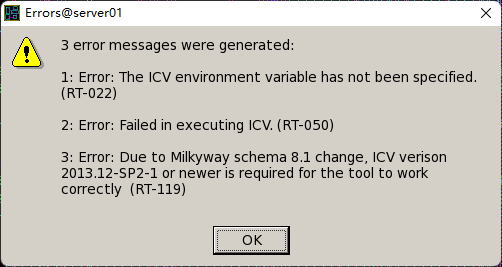
\includegraphics[width=0.9\textwidth]{images/26.png}
    \end{figure}
    \begin{minted}[breaklines]{text}
3 error messages were generated:
1: Error: The ICV environment variable has not been specified. (RT-022)
2. Error: Failed in executing ICV. (RT-050)
3. Error: Due to Milkyway schema 8.1 change, ICV version 2013.12-SP2-1 or newer is required for the tool to work correctly (RT-119)
    \end{minted}
    To check LVS errors, choose Verification > LVS (Figure \ref{f27}).
    \begin{figure}[H]
        \centering
        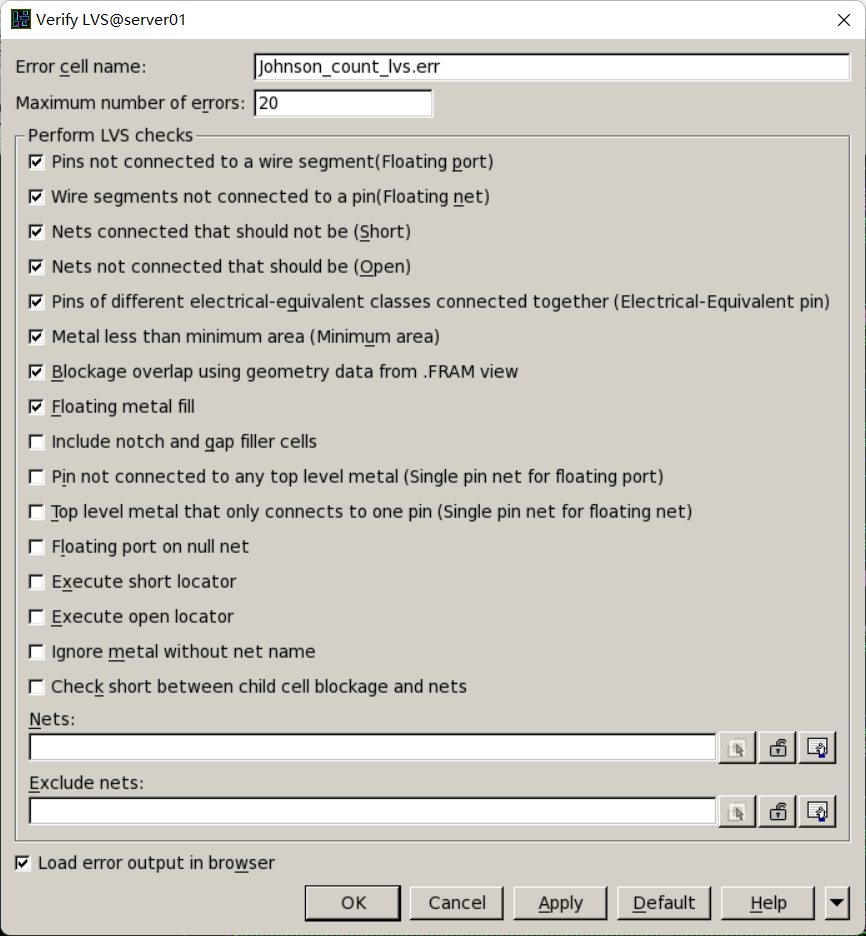
\includegraphics[width=\textwidth]{images/27.png}
        \caption{Check LVS window.}
        \label{f27}
    \end{figure}
    \textit{Take a screenshot of your Error Browser@server01 and a screenshot of your final design view}.
    \item Write the design in the following formats:
    \begin{minted}[breaklines]{text}
icc_shell> write_verilog -pg -no_physical_only_cells ../results/Johnson_count.v
    \end{minted}
    This command generates a Verilog netlist for the current Milkyway design. By specifying \texttt{-pg} and \texttt{-no\_physical\_only\_cells} options.\\
    \texttt{-pg} - Output power and ground nets and ports for all cell instances and module instances.\\
    \texttt{-no\_physical\_only\_cells} - Do not output physical-only cell instances. The same as from the Menu bar,  choose File > Export > Write Verilog... (Figure \ref{f28}).
    \begin{figure}[H]
        \centering
        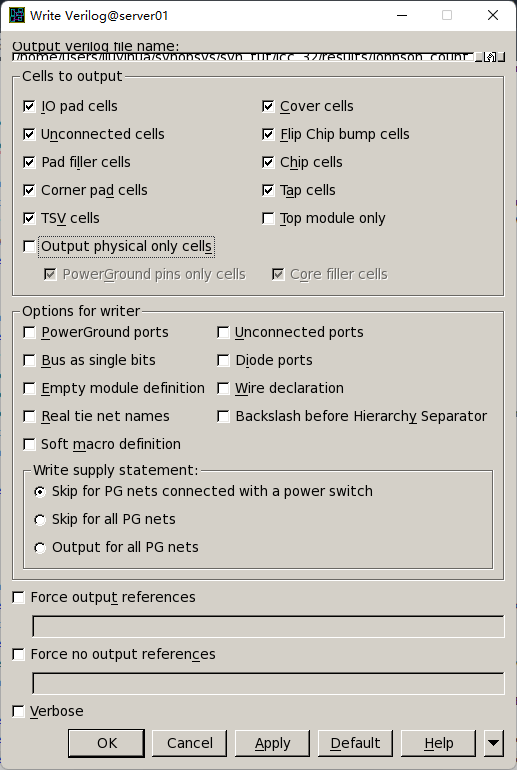
\includegraphics[width=0.8\textwidth]{images/28.png}
        \caption{Write Verilog format box.}
        \label{f28}
    \end{figure}
    To write without PowerGround ports Verilog format the following this command:
    \begin{minted}[breaklines]{text}
icc_shell> write_verilog -pg -no_physical_only_cells ../results/Johnson_count.v
    \end{minted}
    To write the design with Standard Parasitic Exchange Format (SPEF), use the following command:
    \begin{minted}[breaklines]{text}
icc_shell> write_parasitics -output {../results/Johnson_count.spf}
    \end{minted}
    This command writes parasitics for the current design to a disk file.\\
    \texttt{-output}: Specifies the name of the output file to which parasitics for the current design are written.\\
    The same as from the Menu bar, choose File > Export > Write Parasitics (Figure \ref{f29}).
    \begin{figure}[H]
        \centering
        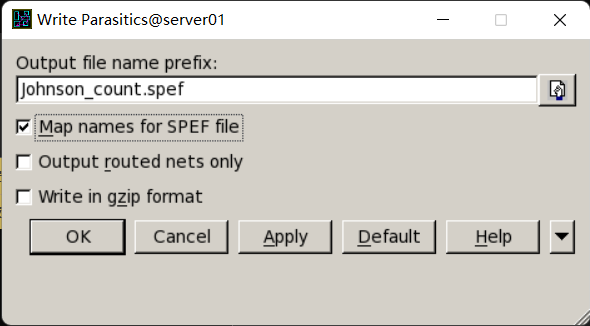
\includegraphics[width=\textwidth]{images/29.png}
        \caption{Write .spef format box.}
        \label{f29}
    \end{figure}
    Command \texttt{write\_stream} writes the data in the specified library to a file in GDS format. The options are set by \texttt{set\_write\_stream\_options}.
    \begin{minted}[breaklines]{tcl}
set_write_stream_options -map_layer ../ref/saed90nm.gdsout.map -output_filling fill	-child_depth 20	-output_outdated_fill -output_pin {text geometry}
write_stream -lib COUNT -format gds -cells Johnson_count ../results/Johnson_count.gds
    \end{minted}
    \texttt{-map\_layer} Specifies the file that defines the layer mapping from Milkyway to GDSII.\\
    \texttt{-output\_filling} Specifies the types of filling data to output.\\
    \texttt{-child\_depth 20} Specifies the hierarchical level to output child cells. To export all child cells, specify a large number, such as 20.\\
    \texttt{-output\_outdated\_fill} Forces the output of fill data even if the fill data is out-of-date.\\
    \texttt{-output\_pin} Specifies the object types to output for each pin.\\
    The same as from the Menu bar, choose File > Export > Write Stream (Figure \ref{f30}).
    \begin{figure}[H]
        \centering
        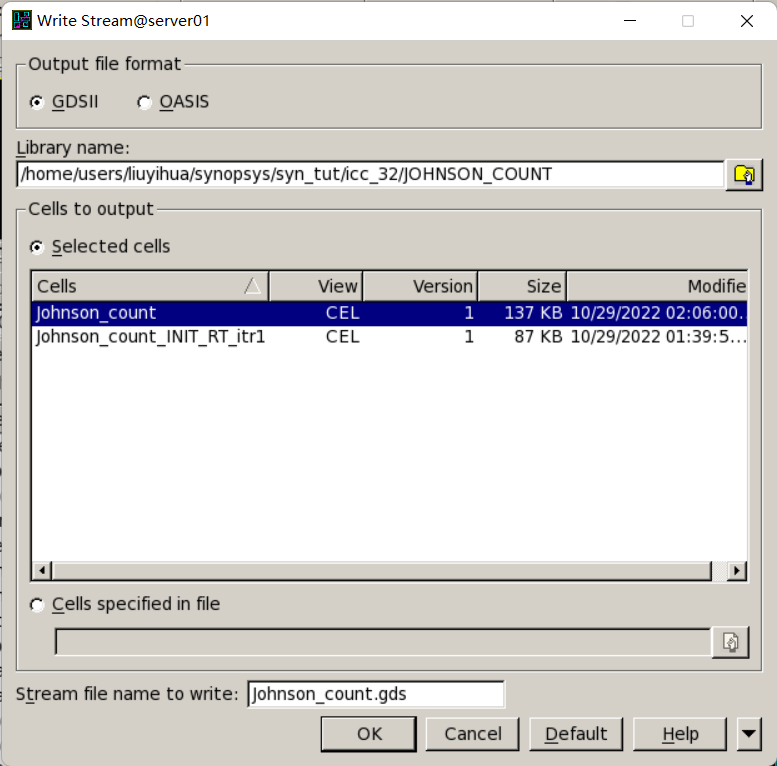
\includegraphics[width=\textwidth]{images/30.png}
        \caption{Write .gds format box.}
        \label{f30}
    \end{figure}
    In this design, output results are stored in ../.location/results/ directory.
    \item To exit IC Compiler write exit in the command line.
    \begin{minted}[breaklines]{text}
exit
    \end{minted}
\end{enumerate}

\newpage
\section{Formal Verification}\label{SFV}
\subsection{Introduction}
The purpose of Formality is to detect unexpected differences that may have been introduced into a design during development.

For this lab, you need to copy \texttt{/home/Flow/Synopsys/Scripts/formality\_32} to the \texttt{syn\_tut} directory.
\begin{minted}[breaklines]{bash}
cd ~/synopsys/syn_tut
cp -r /home/Flow/Synopsys/Scripts/formality_32/ .
cd formality_32
cd pre_lay
\end{minted}
Before we start Formality, we're going to create a link to the database that we'll be using (we'll need this later). To create this link, navigate to the scripts directory and run the \texttt{link\_to\_database.sh} script:
\begin{minted}{bash}
cd scripts
./link_to_database.sh
\end{minted}
\textit{You may need to modify the script if needed. In this lab, we will use Synopsys Formality (R) Version R-2020.09-SP3 for linux64}.

To start Formality (as usual use the work directory), enter the following command at the terminal (here we verify the prelayout netlist, for postlayout you just need to use the postlay directory):
\begin{minted}{bash}
cd ../work
fm_shell
\end{minted}
The \texttt{fm\_shell} command starts the Formality shell environment. From here, start the graphical user interface (GUI) as follows:
\begin{minted}{text}
fm_shell (setup)> start_gui
\end{minted}
Alternatively, To Start Formality in GUI mode you can also enter:
\begin{minted}{bash}
fm_shell -gui
\end{minted}
This opens the Formality top-level GUI window.
\begin{figure}[H]
    \centering
    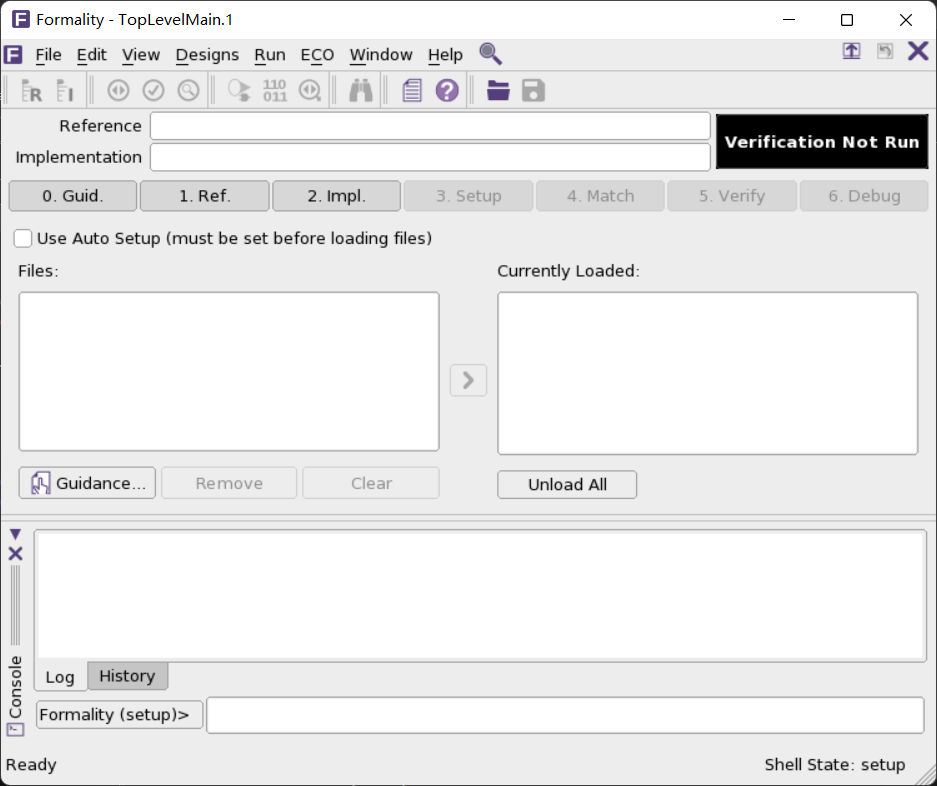
\includegraphics[width=\textwidth]{images/40.png}
    \caption{The Main Window of Formality GUI.}
\end{figure}
In Formality, the following concepts are used:
\begin{itemize}
    \item Reference design: This design is the golden design, the standard against which Formality tests for equivalence.
    \item Implementation design: This design is the changed design. It is the design whose correctness you want to prove. For example, a newly synthesized design is an implementation of the source RTL design.
    \item The setup indicates the mode that is currently in when using commands. The modes are "setup", "match", and "verify".
\end{itemize}
When Formality is invoked, begin in the setup mode.
\subsection{Tasks}
If Formality is given the result of DC, then work in the \texttt{pre\_lay} directory, and if Formality is given the result of ICC, then work in the \texttt{post\_lay} directory.

This lab is an example where Formality works with the result of DC. Therefore, use the \texttt{pre\_lay} directory. Running Formality with the result of ICC is similar to running these lab steps.

To understand Formality's general sections, you can also execute the commands step-by-step (recommended for first-time users).
\subsubsection{Guidance (Load Automated Setup File)}
Before specifying the reference and implementation designs, you can optionally load an automated setup file (.svf) into Formality. The automated setup file helps Formality process design changes caused by other tools used in the design flow. Formality uses this file to assist the compare point matching and verification process. For each automated setup file that is loaded, Formality processes the content and stores the information for use during the name-based compare point matching period.

For this Lab, let us Load the \texttt{default.svf} file.
\begin{enumerate}
    \item In "0. Guid." click Guidance...
    \item Locate the \texttt{default.svf} file within the Source Directory
    \item Click Open
    \item Click the right arrow button to load files
\end{enumerate}
\begin{figure}[H]
    \centering
    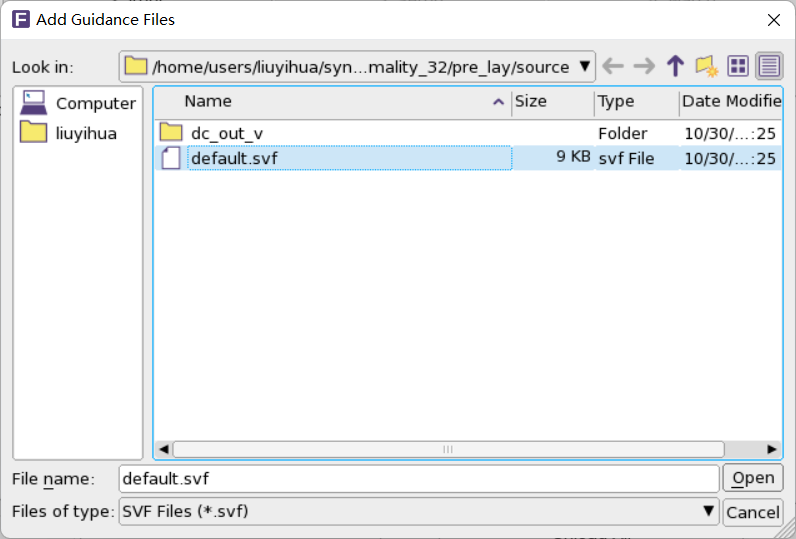
\includegraphics[width=\textwidth]{images/41.png}
    \caption{Loading Guidance.}
\end{figure}
\begin{minted}[breaklines,breakanywhere]{tcl}
set_svf -append { /home/users/<username>/synopsys/syn_tut/formality_32/pre_lay/source/default.svf }
\end{minted}
\subsubsection{Reference (Specify the Reference Design)}
Specifying the reference design involves the reading in of design files, optionally reading in technology libraries, and setting the top-level design. The reference design is the design with which the transformed (implementation) design is compared. Click the "1. Ref." Tab
\begin{enumerate}
    \item \textbf{Source the Design Entity}\\
    During this stage of Reference, the files that describe the entirety of the Reference Design will be loaded by Formality.
    \begin{enumerate}
        \item In the "1. Read Design Files" tab, in the Verilog tab, in the Preferences frame, select WORK as the Design Library and select the correct Verilog Version, then click Verilog...
        \item Locate the \texttt{Johnson\_count.v} File within the Source Directory
        \item Click Open
        \item Click the right arrow button to load files
    \end{enumerate}
    \begin{figure}[H]
        \centering
        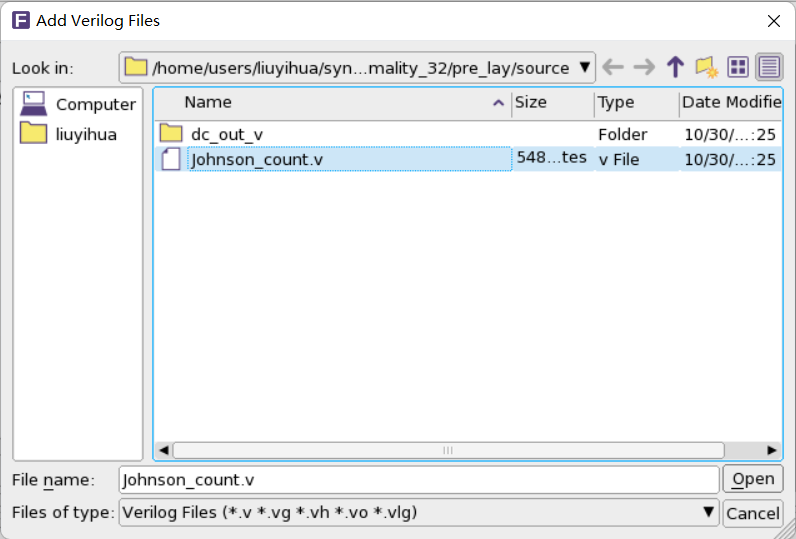
\includegraphics[width=\textwidth]{images/42.png}
        \caption{Set up RTL Source.}
    \end{figure}
    \begin{minted}[breaklines,breakanywhere]{tcl}
read_verilog -container r -libname WORK -05 { /home/users/<username>/synopsys/syn_tut/formality_32/pre_lay/source/Johnson_count.v } 
    \end{minted}
    \item \textbf{Source the DB file}\\
    During this stage of Reference, an optional technology library may be loaded for Formality, and the design, to use.
    \begin{enumerate}
        \item Select the "2. Read DB Libraries" Tab within "1. Ref."
        \item In the Preferences frame, select WORK as the Design Library, check "Determined by DB" and "Read as a shared library". Click DB...
        \item Locate \texttt{database\_link.db} within the \texttt{ref/} directory. This is the link to the database that we created earlier.
        \item Click Open
        \item Click the right arrow button to load files
    \end{enumerate}
    \begin{figure}[H]
        \centering
        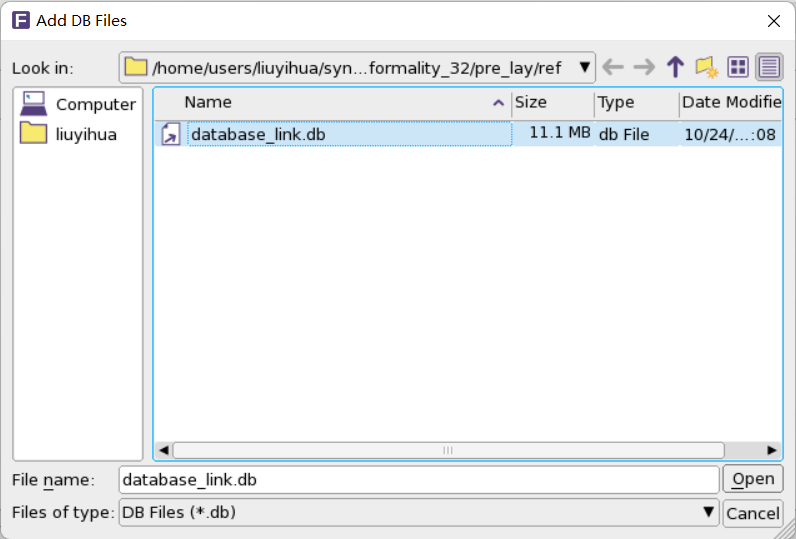
\includegraphics[width=\textwidth]{images/43.png}
        \caption{Setting the DB File.}
    \end{figure}
    \begin{minted}[breaklines,breakanywhere]{tcl}
read_db { /home/users/<username>/synopsys/syn_tut/formality_32/pre_lay/ref/database_link.db } 
    \end{minted}
    \item \textbf{Set Top Design of reference}\\
    During this stage of Reference, the Top Level Design of the Reference Entity loaded earlier will be set.
    \begin{enumerate}
        \item Select the "3. Set Top Design" Tab within "1. Ref."
        \item Select the Library WORK under "1. Choose a Library"
        \item Select \texttt{Johnson\_count} under "2. Choose a Design"
        \item Click "Set Top" under "3. Set and link the top design"
    \end{enumerate}
    \begin{figure}[H]
        \centering
        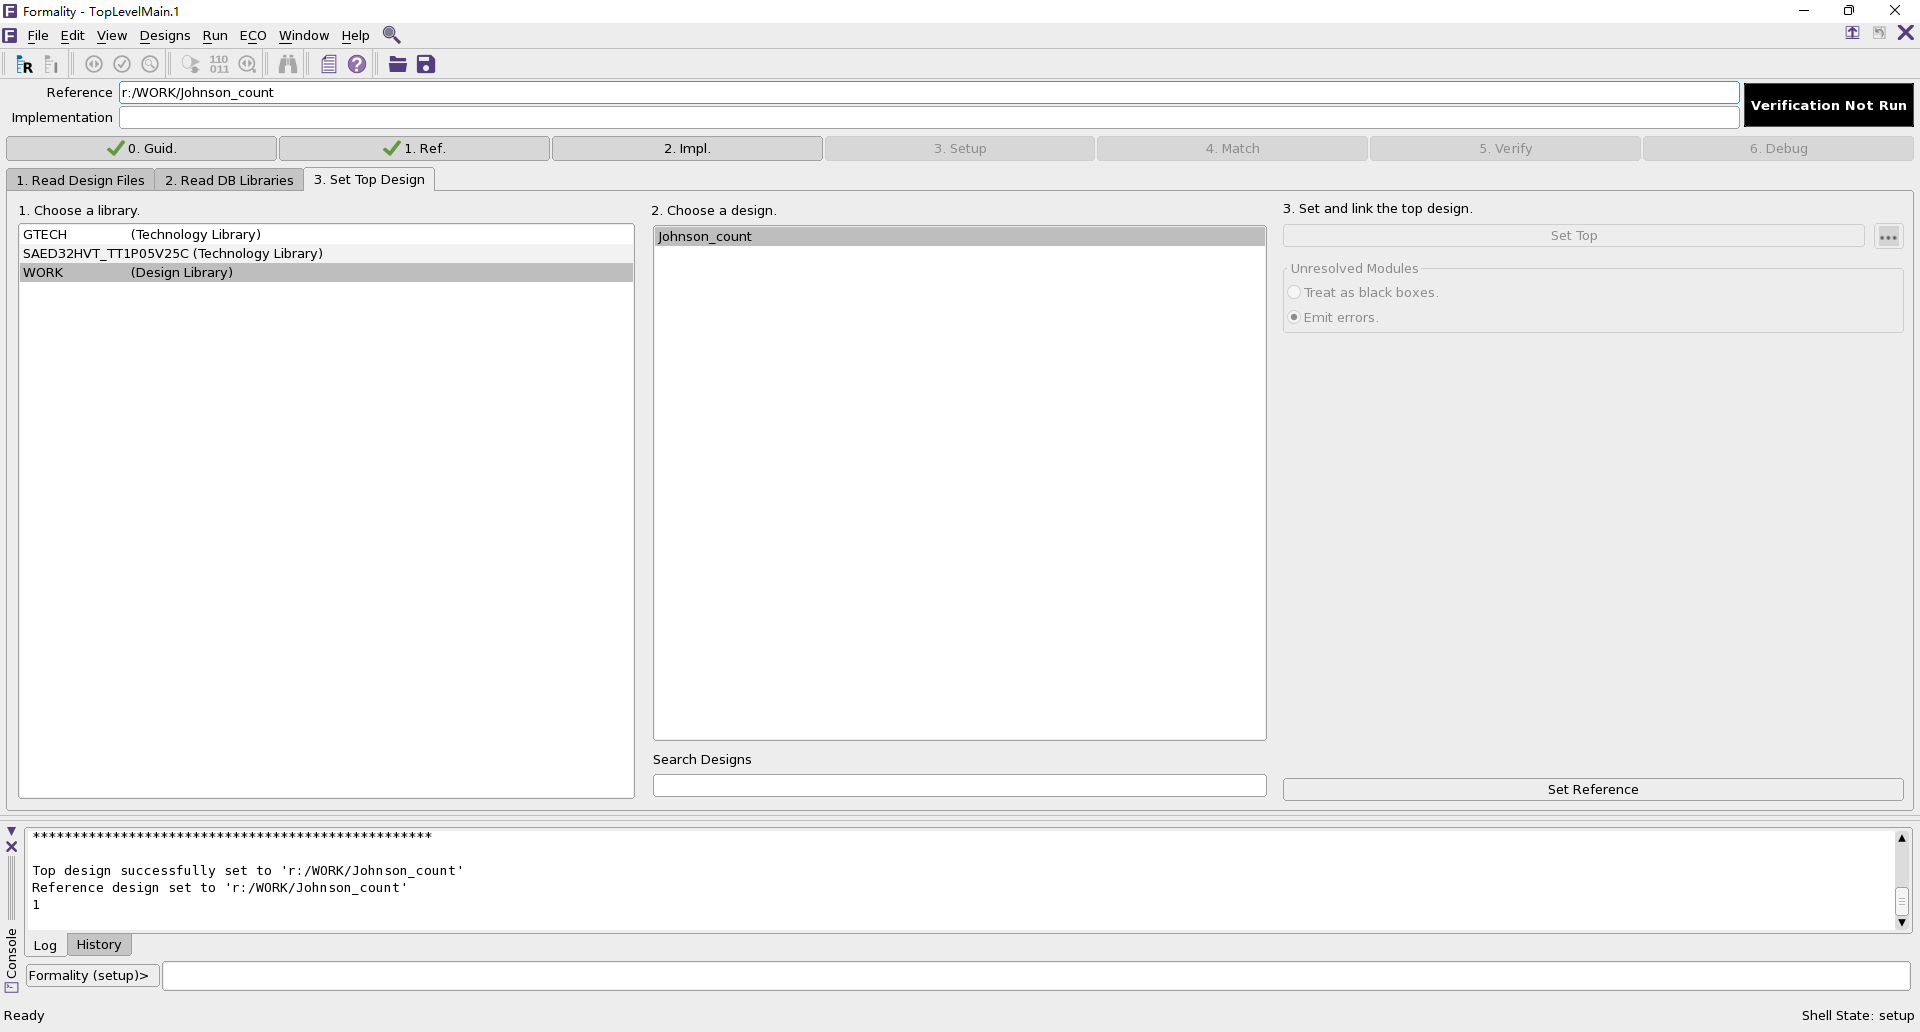
\includegraphics[width=\textwidth]{images/44.png}
        \caption{Setting the Top Level Design.}
    \end{figure}
    \begin{minted}{tcl}
set_top r:/WORK/Johnson_count
    \end{minted}
\end{enumerate}
\subsubsection{Implementation (Specify the Implementation Design)}
The procedure for specifying the implementation design is identical to that for specifying the reference design. The implementation design is the gate-level netlist after the design is compiled. Click the "2. Impl." Tab
\begin{enumerate}
    \item \textbf{Source the Implementation Design}\\
    During this stage of Implementation, the files that describe the entirety of the Compiled Design will be loaded by Formality.
    \begin{enumerate}
        \item In the Verilog tab, in the Preferences frame, select WORK as the Design Library and select the correct Verilog Version, then click Verilog...
        \item Locate the \texttt{Johnson\_count\_dc.v} file within \texttt{source/dc\_out\_v}
        \item Click Open
        \item Click the right arrow button to load files
    \end{enumerate}
    \begin{figure}[H]
        \centering
        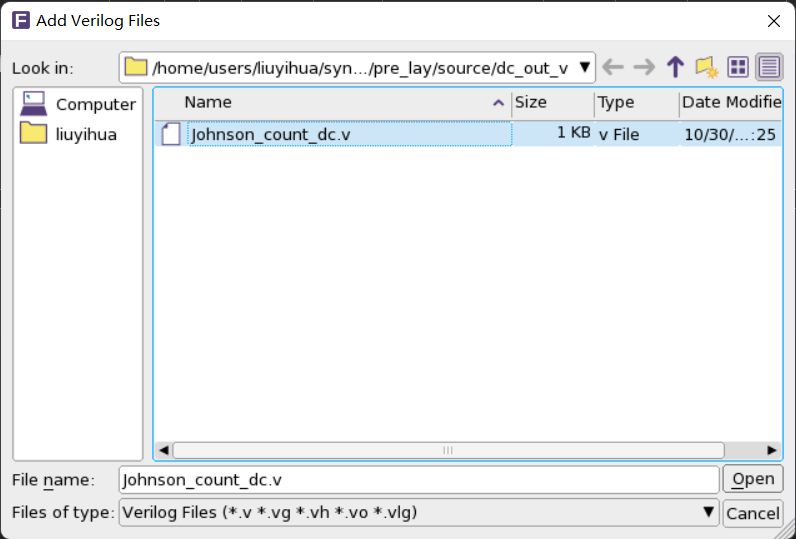
\includegraphics[width=\textwidth]{images/45.png}
        \caption{Set Gate Level Verilog.}
    \end{figure}
    \begin{minted}[breaklines,breakanywhere]{tcl}
read_verilog -container i -libname WORK -05 { /home/users/<username>/synopsys/syn_tut/formality_32/pre_lay/source/dc_out_v/Johnson_count_dc.v } 
    \end{minted}
    \item \textbf{Source the DB file}\\
    During this stage of Implementation, we will be loading the technology library for use by design, the same as the "1. Ref." Stage.
    \item \textbf{Set Top Design of reference}\\
    During this stage of Implementation, the Top Level Design of the Compiled Entity is loaded, the same as the "1. Ref." Stage.
    \begin{minted}{tcl}
set_top i:/WORK/Johnson_count
    \end{minted}
\end{enumerate}
\subsubsection{Setup (Setup the Design)}
After Importing the Reference and Implementation Design, Formality is then Set up for the Comparison between the two. Click the "3. Setup" tab.

Now we add the reference and implementation constants.
\begin{enumerate}
    \item Click Set...
    \item Select Input Ports under the Reference Tab\\
    You should now see four ports appear underneath the Instance of the Design\\
    \textit{Note that the new version changed the "Hide Objects" frame to "Show Objects" frame}.
    \item Select the SE port
    \item Click Apply
    \item Repeat process for the r port as well as SE and r under the implementation Tab
\end{enumerate}
\begin{figure}[H]
    \centering
    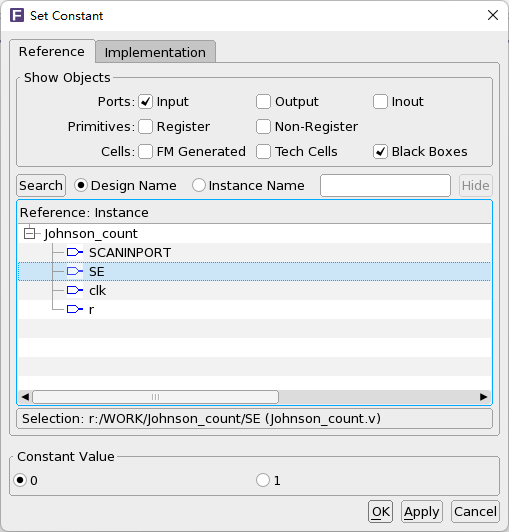
\includegraphics[width=\textwidth]{images/46.png}
    \caption{Setup the Design Window.}
\end{figure}
\begin{minted}{tcl}
set_constant -type port r:/WORK/Johnson_count/SE 0 
set_constant -type port r:/WORK/Johnson_count/r 0 
set_constant -type port i:/WORK/Johnson_count/SE 0 
set_constant -type port i:/WORK/Johnson_count/r 0
\end{minted}
\begin{figure}[H]
    \centering
    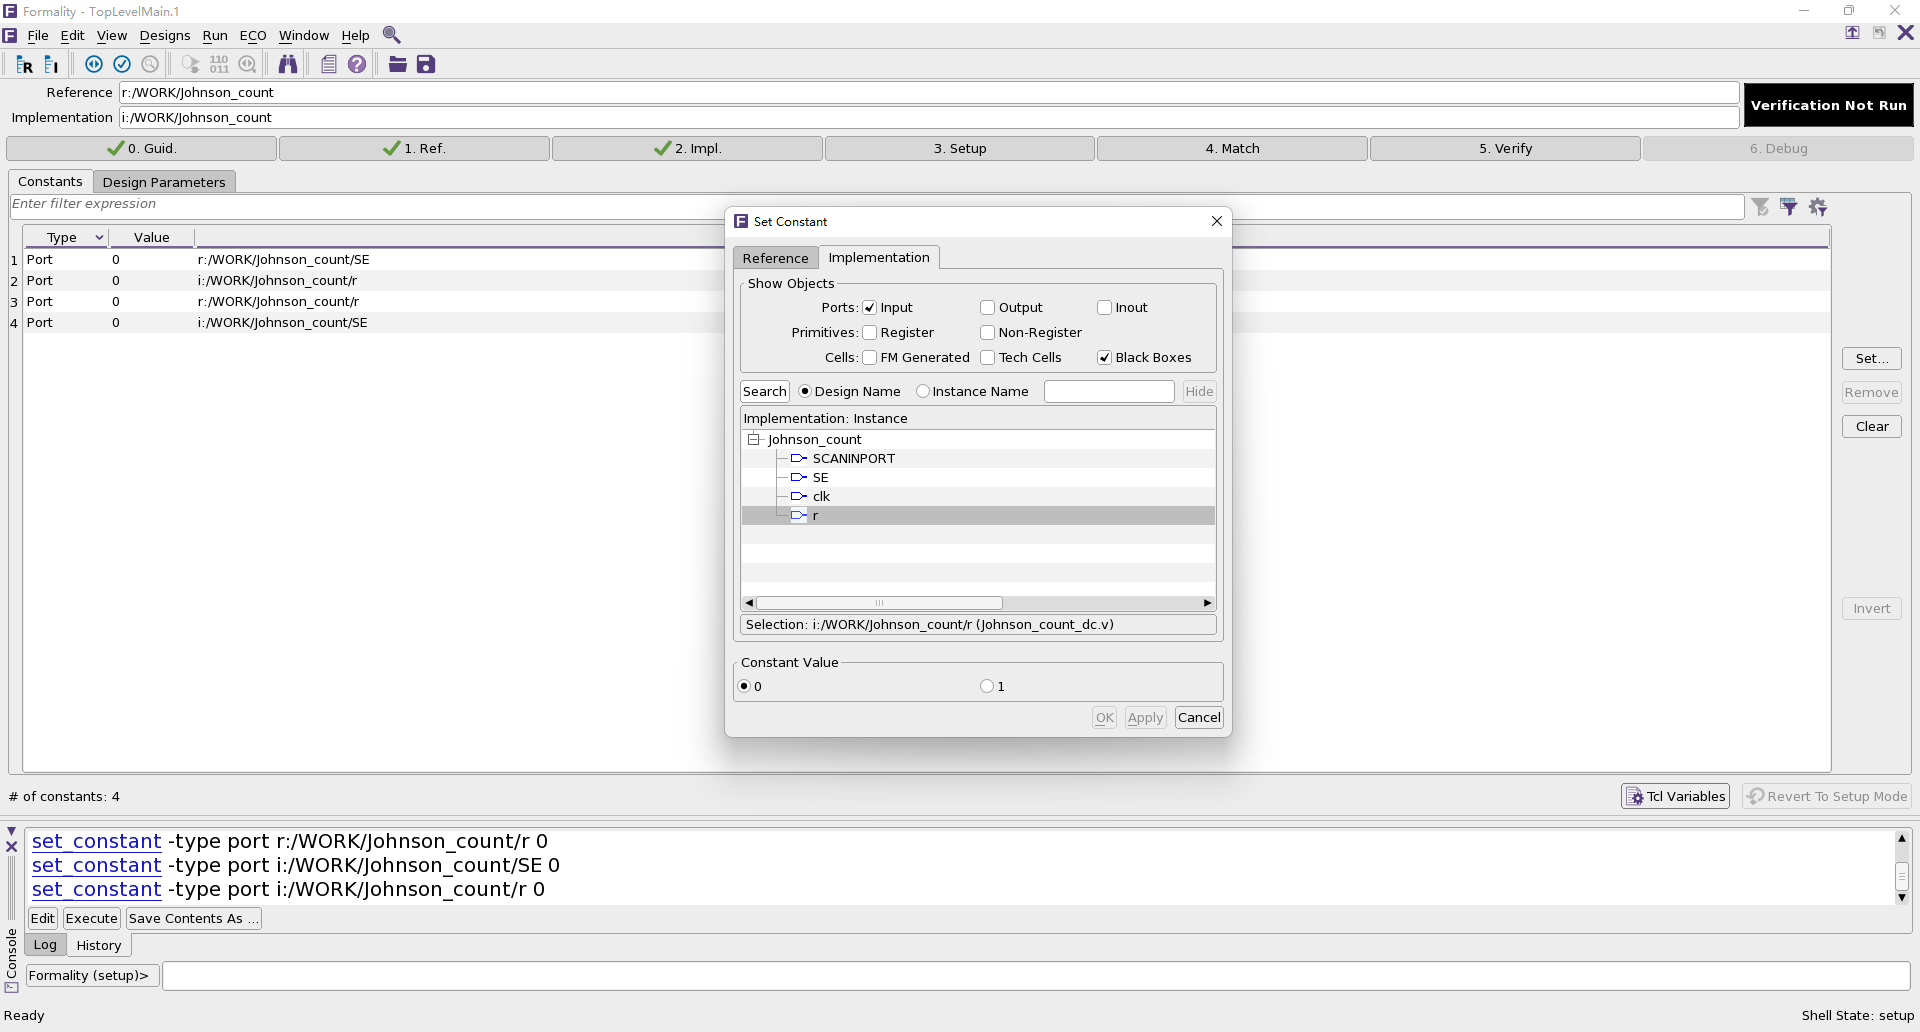
\includegraphics[width=0.9\textwidth]{images/47.png}
    \caption{After setting up the Design.}
\end{figure}
\subsubsection{Match (Match Compare Points)}\label{SMatch}
"Match compare points" is the process by which Formality segments the Reference and Implementation Designs into logical units called logic cones. To match compare points between \texttt{Johnson\_count.v} and \texttt{Johnson\_count\_dc.v} (after DC), do the following:
\begin{enumerate}
    \item Click upon the "4. Match" Tab to start the Matching Process
    \item Click Run Matching
\end{enumerate}
\begin{figure}[H]
    \centering
    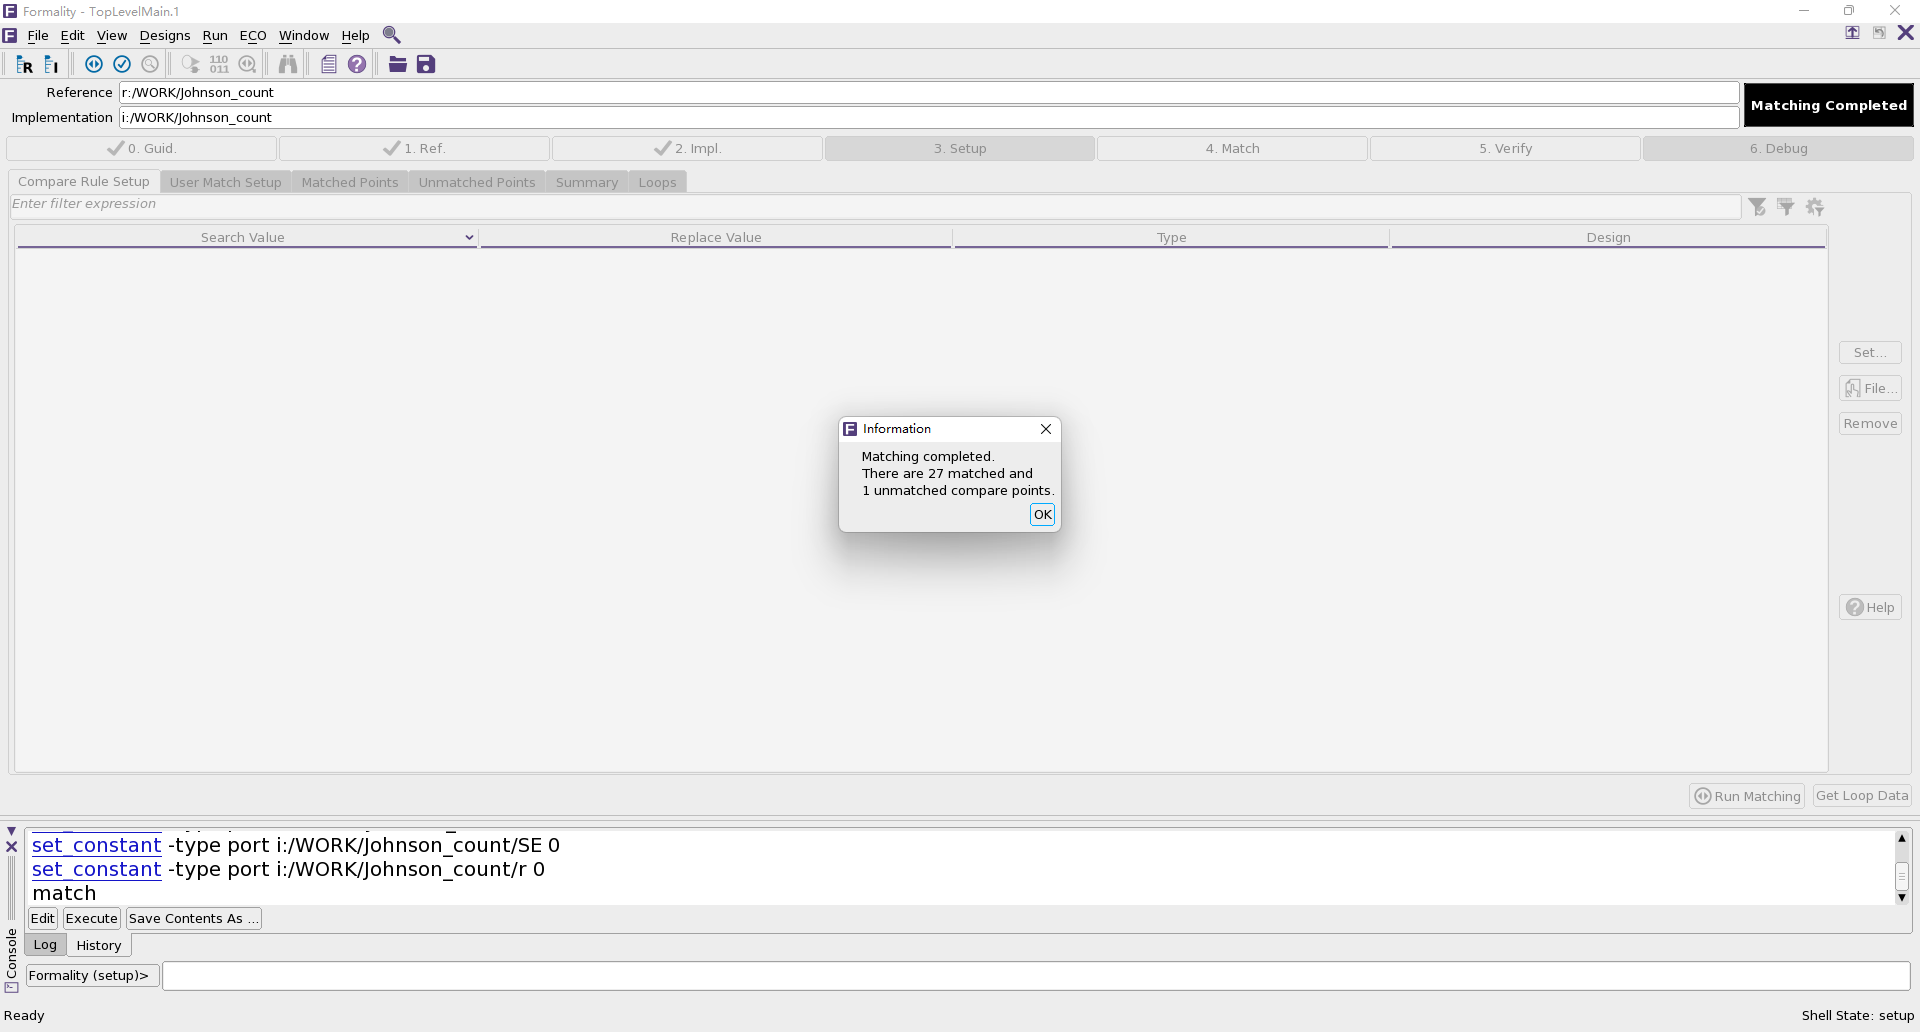
\includegraphics[width=0.9\textwidth]{images/48.png}
    \caption{Match compare points.}
\end{figure}
\begin{minted}{tcl}
match
\end{minted}
As seen, Formality matches the logic cones between each Design for later Comparison and Verification. As can be seen, we have one unmatched point between our two implementations. This indicates the designs do not use the same input and output ports or registers, some of the ports are undriven or have similar issues.
\begin{enumerate}
    \item To see the unmatched points, click the Unmatched Points tab.\\
    Here we can see our unmatched point.
    \item Right Click on the only Reference Object
    \item Click View Reference Object\\
    Here we can see our unmatched point seems to be an undriven port. Zooming out, we can see the entire Reference Design.
    \item Closing the Design, Right Click on the Object, and Click View Reference Source\\
    Here we can see the reference object does not utilize the SCANOUTPORT Output.
\end{enumerate}
\begin{figure}[H]
    \centering
    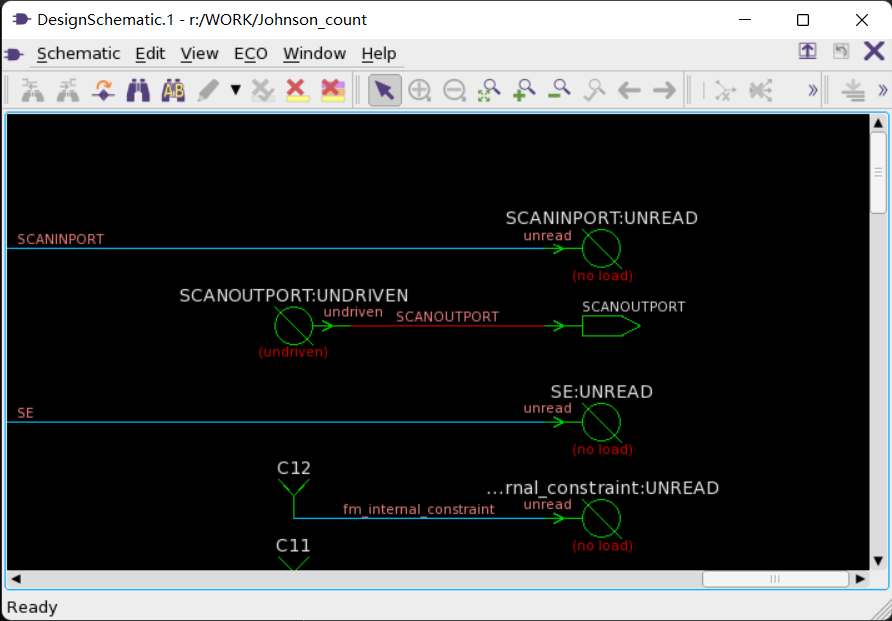
\includegraphics[width=\textwidth]{images/49.png}
    \caption{Unmatched Point.}
\end{figure}
\begin{figure}[H]
    \centering
    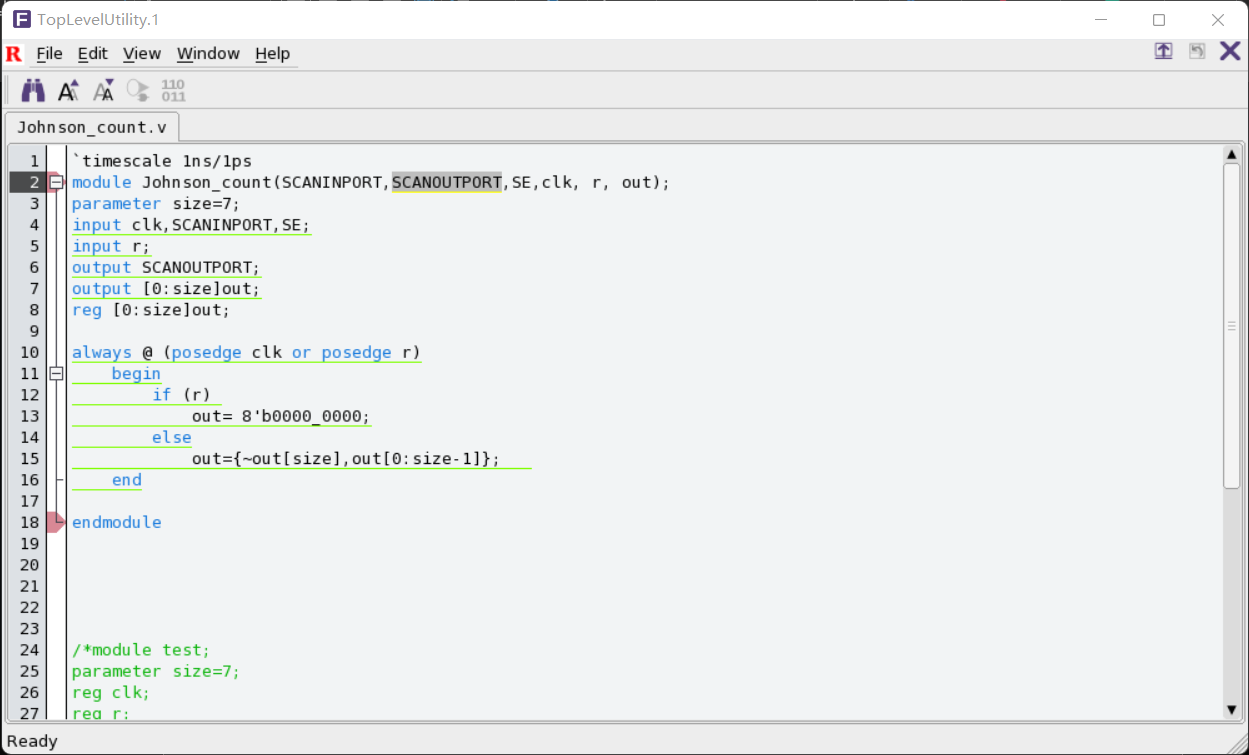
\includegraphics[width=\textwidth]{images/50.png}
\end{figure}
From here, we may continue to verify and debug, which will fail due to our undriven signal. If continued, one may look upon both the Reference and Implementation Design Objects and Sources to look at the differences between the two designs. As seen in Matching, we have an undriven signal, so driving the signal will remedy the issue.
\begin{enumerate}
    \item Open a New Terminal
    \item Navigate to \texttt{Johnson\_count.v} in \texttt{pre\_lay/source}
    \item Run \texttt{gedit Johnson\_count.v}
    \item Add an instance \texttt{NBUFFX2\_HVT U12} in the Empty Line Before \texttt{endmodule}
    \item Save the file
\end{enumerate}
% \begin{figure}[H]
%     \centering
%     \includegraphics[width=\textwidth]{images/51.png}
%     \caption{Modified File.}
% \end{figure}
After this, you must go through Reference, Setup, and Match again to Reload the Modified File and Set it up for Verification. After Doing so, when Running Match, no Unmatched Points will appear.
\subsubsection{Verify (Verify the Designs)}\label{SVerify}
When using the verify command, Formality attempts to prove design equivalence between an implementation design and a reference design. This section describes how to verify a design or a single compare point, as well as how to perform traditional hierarchical verification.

Click on the "5. Verify" Tab, Then Click on Verify.
\begin{figure}[H]
    \centering
    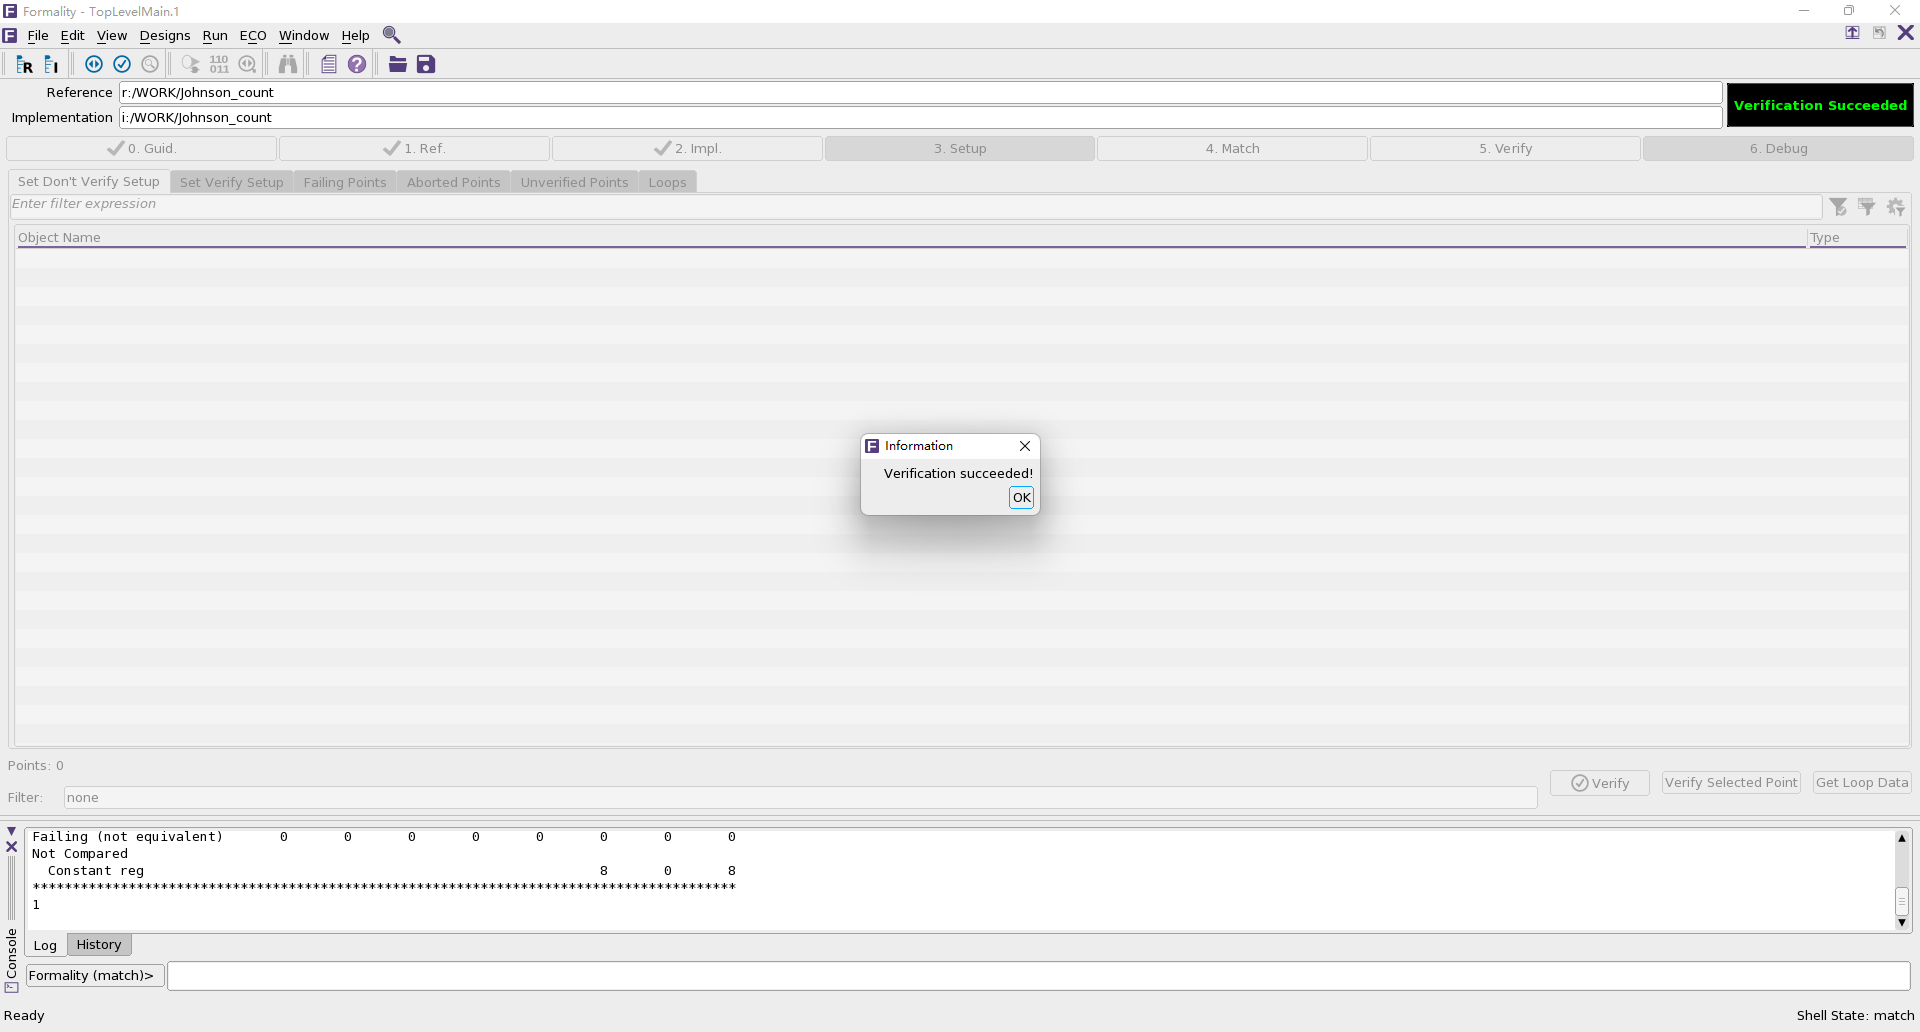
\includegraphics[width=\textwidth]{images/52.png}
    \caption{Verify the design.}
\end{figure}
\begin{minted}{tcl}
verify
\end{minted}
The verifying process was finished successfully.

Should Verification Fail, ensure that you have updated the reference design, so no more undriven ports exist and the new design has been loaded.

Ensure Setup and Match were Run as well after doing this.

Should "'set\_constant' can only be executed in SETUP mode" appear or similar issues, type setup in the formality terminal or command line and attempt the step again.
\begin{minted}{text}
Formality (match)> setup or Formality (verify)> setup or etc.
\end{minted}
\subsubsection{Debug}\label{SDebug}
After Verify is run, if any issues are found, one must find the exact points in the designs that exhibit the difference in functionality and then fix them during this Debugging Stage.
\begin{figure}[H]
    \centering
    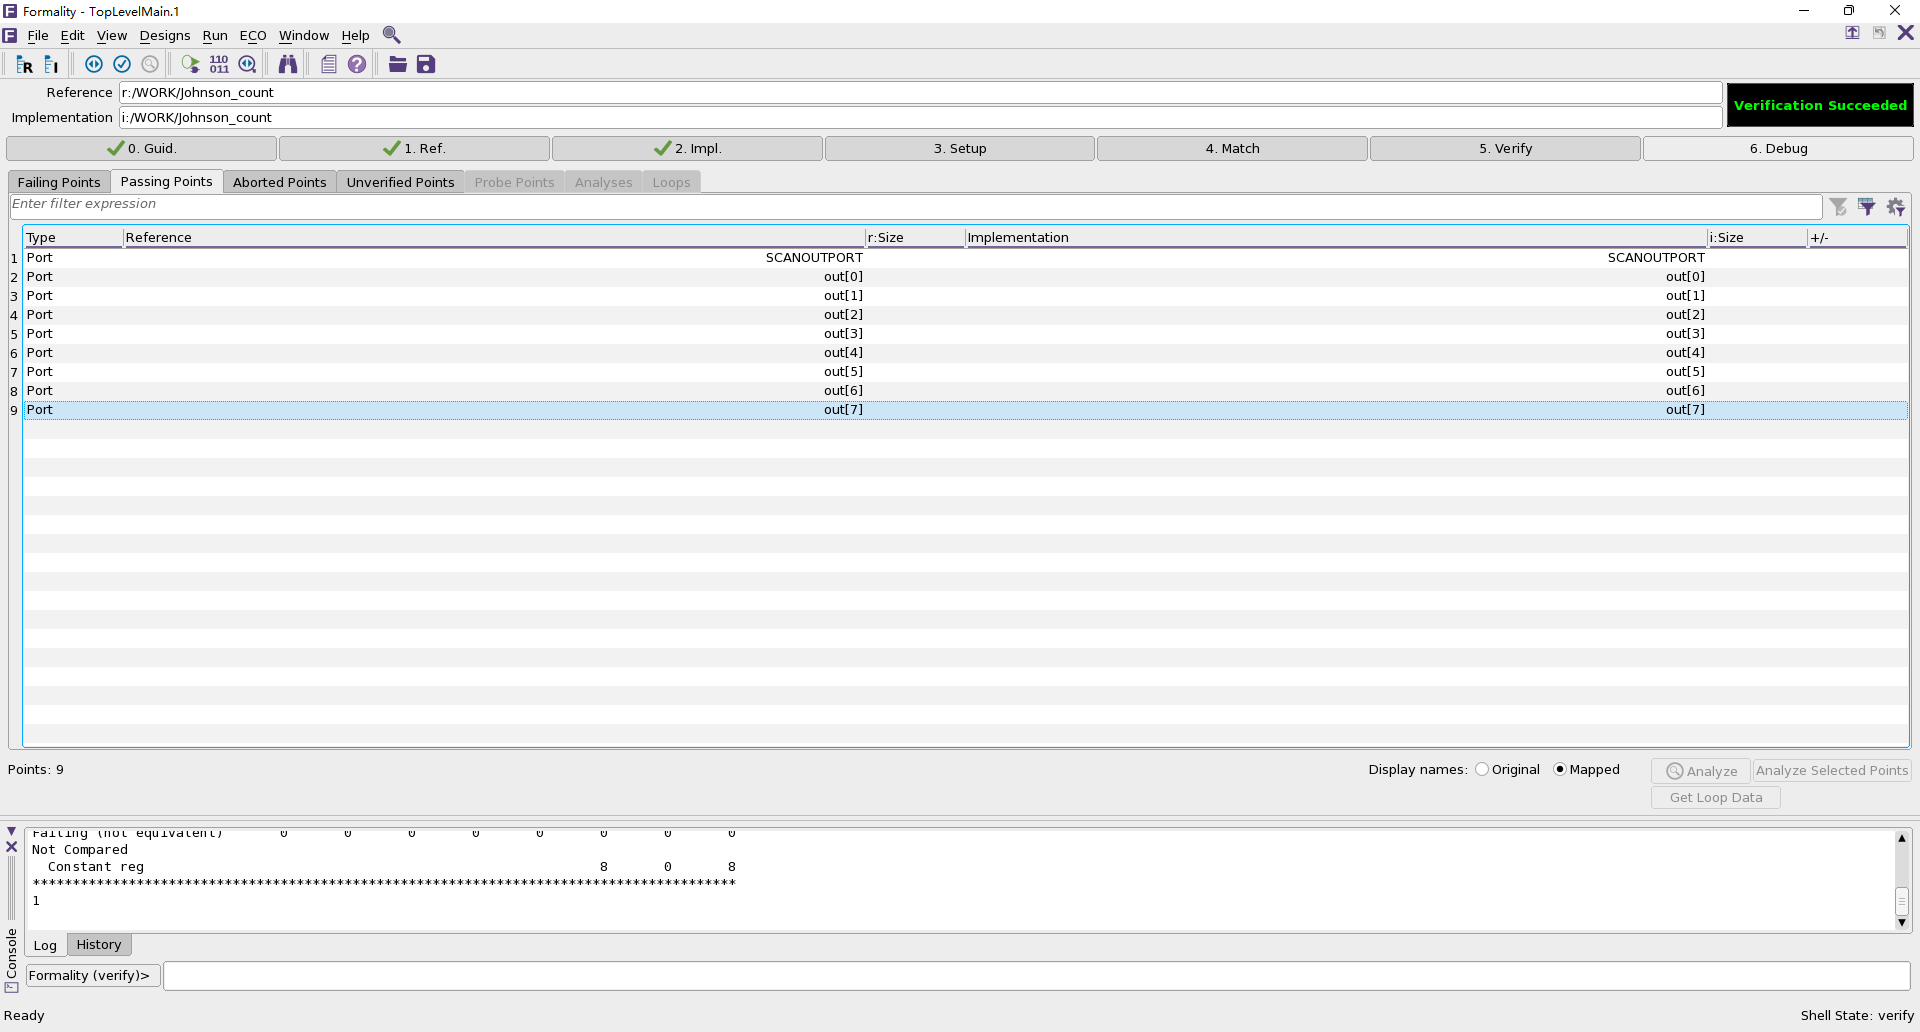
\includegraphics[width=\textwidth]{images/53.png}
    \caption{Debugging the Design.}
\end{figure}
Formality is able to simultaneously display Reference and Implementation Source Views and mark differences and/or similarities. This is done by right-clicking on the object and Clicking View Reference/Implementation Source.
\begin{figure}[H]
    \centering
    \begin{subfigure}{\textwidth}
        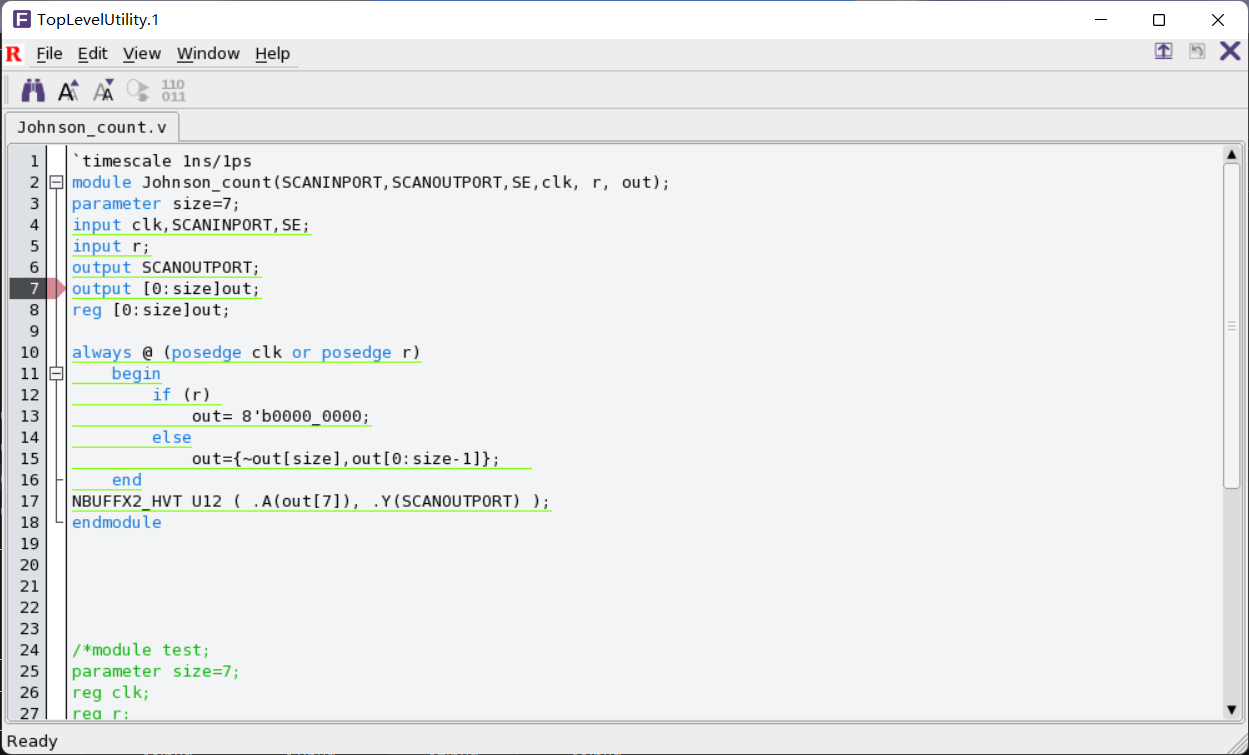
\includegraphics[width=\textwidth]{images/54.png}
        \subcaption{Pre-lay}
    \end{subfigure}
\end{figure}
\begin{figure}[H]\ContinuedFloat
    \centering
    \begin{subfigure}{\textwidth}
        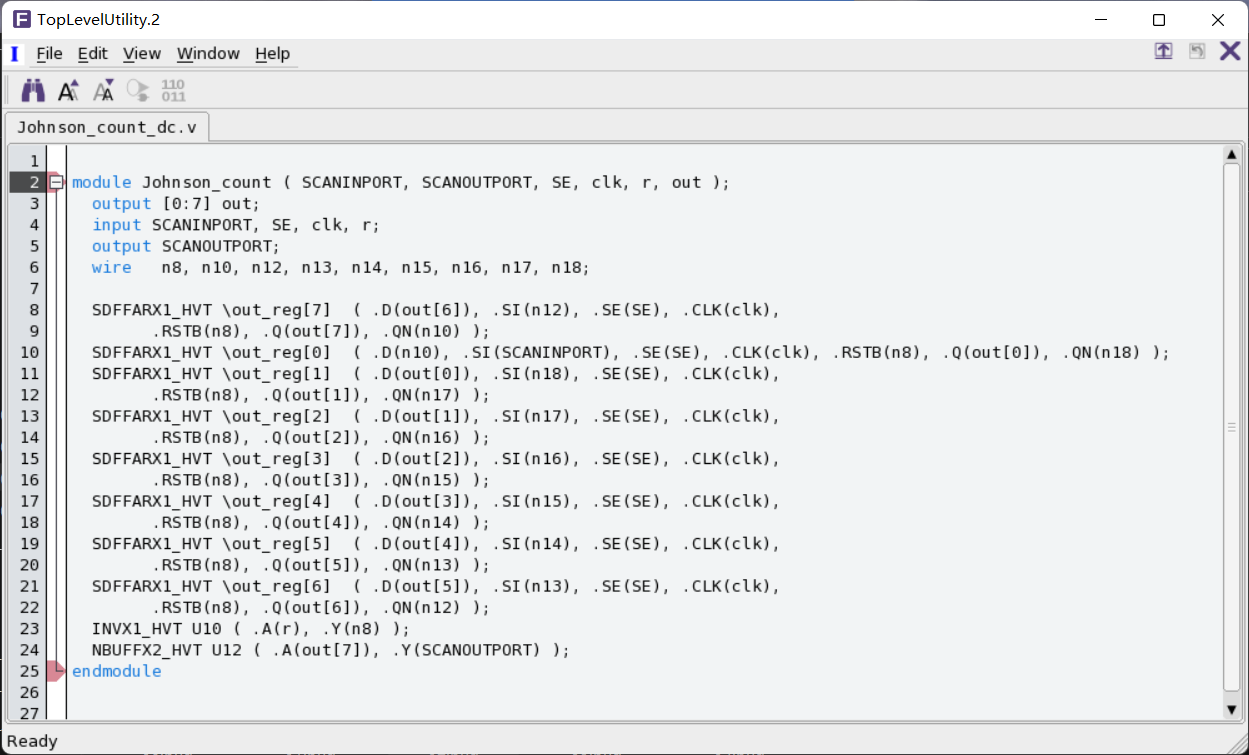
\includegraphics[width=\textwidth]{images/55.png}
        \subcaption{Post-lay}
    \end{subfigure}
    \caption{Implementation and Reference Verilog}
\end{figure}
Formality can also display a schematic view and highlight reference objects on it. This is done in a similar manner to the sources except clicking View Reference/Implementation Source.
\begin{figure}[H]
    \centering
    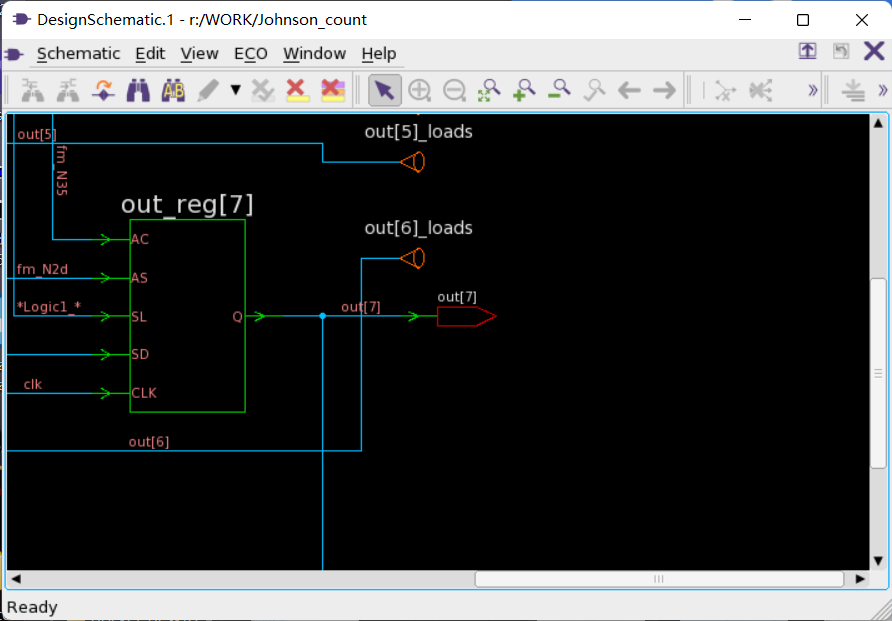
\includegraphics[width=0.8\textwidth]{images/56.png}
    \caption{View Reference Object in the schematic.}
\end{figure}
In this lab work, design output results are stored in the \texttt{../results/} directory.

To exit Formality write exit in the command line.
\begin{minted}{text}
Formality (verify)> exit
\end{minted}

\newpage
% \section{Formal Verification}
% The purpose of Formality is to detect unexpected differences that may have been introduced into a design during development. For this tutorial, you need to download the formality\_32.zip file (attached at the end of the wiki page) and unzip it in the syn\_tut directory.
\section{Static Timing Analysis with PrimeTime}\label{SSTA}
\subsection{Introduction}
PrimeTime is a full-chip, gate-level Static Timing Analysis (STA) tool that is an essential part of the design and analysis flow for today's large-chip designs.

Why is timing analysis important when designing a chip?

Timing is important because just designing the chip is not enough; we need to know how fast the chip is going to run, how fast the chip is going to interact with the other chips, how fast the input reaches the output etc.

Timing Analysis is a method of verifying the timing performance of a design by checking for all possible timing violations in all possible paths.
\subsection{PrimeTime Basic Flow}
\begin{figure}[H]
    \centering
    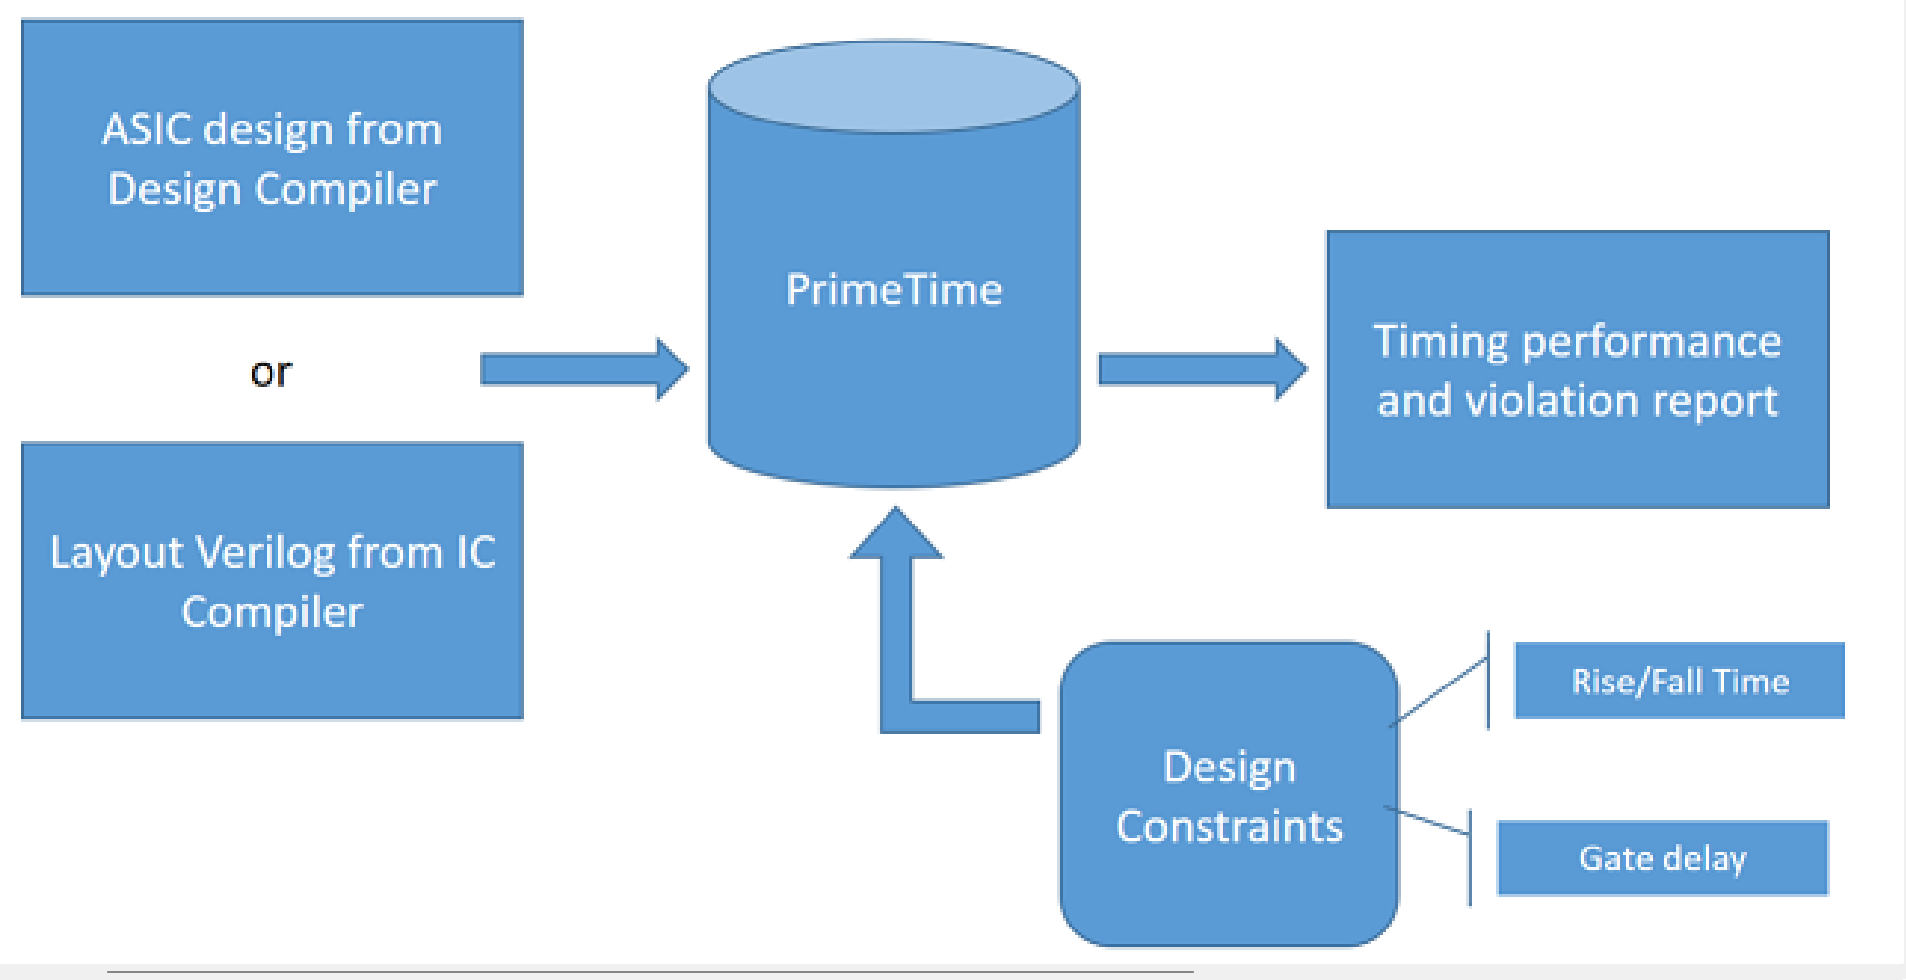
\includegraphics[width=\textwidth]{images/31.png}
\end{figure}
PrimeTime can be used to perform STA using either the results of the Design Compiler (DC) or Integrated Circuit Compiler (ICC). If the DC results are used, we are doing pre-layout STA. If the ICC results are used, we are doing post-layout STA. PrimeTime accepts as input a Verilog file from the DC or ICC and then a design constraints file specifying the timing constraints of the design. With these inputs, PrimeTime produces timing performance and
violation reports.

If you are using results from the Design Compiler, then work in the \texttt{pre\_lay} directory. If you are using results from the IC Compiler, then work in the \texttt{post\_lay} directory. This lab will go through pre-layout STA first and then post-layout STA. \textit{In this lab, we will use Synopsys PrimeTime (R) Version R-2020.09-SP1 for linux64}.
\subsection{Pre-Layout STA}\label{SPreSTA}
\begin{enumerate}
    \item Unzip the \texttt{/home/Flow/Synopsys/Scripts/pt\_32.zip} file to the \texttt{syn\_tut} directory. Now, set up the Synopsys tools and start the PrimeTime graphical user interface (GUI) by entering the following:
    \begin{minted}[breaklines]{bash}
cd ~/synopsys/syn_tut
unzip /home/Flow/Synopsys/Scripts/pt_32.zip -d .
cd pt_32
cd pre_lay
cd work
pt_shell -gui
    \end{minted}
    This opens the PrimeTime top-level GUI window (Figure \ref{f32}).
    \begin{figure}[H]
        \centering
        \includegraphics[width=\textwidth]{images/32.png}
        \caption{PrimeTime Top-level GUI window.}
        \label{f32}
    \end{figure}
    If it shows an error:
    \begin{minted}[breaklines]{text}
Error: Library Compiler executable path is not set. (PT-063)
    \end{minted}
    and quitted with error:
    \begin{minted}[breaklines]{text}
Suppressed Messages Summary:
Id          Severity      Occurrences   Suppressed
-------------------------------------------------------------------------------
CMD-005     Error                  12           12
Total 1 type of message is suppressed
    \end{minted}
    Please read Appendix: Troubleshooting \ref{ALC}.
    \item The paths to the libraries are set up by running the setup.tcl file in the scripts directory. Look at this file using your text editor of choice to see how the libraries are being set up \textit{and make modifications if needed}. To run the script, enter the following command into PrimeTime:
    \begin{minted}{text}
pt_shell> source ../scripts/setup.tcl
    \end{minted}
    \item Next, notice that there is one other script in the scripts directory named \texttt{sta\_pre\_lay.scr}. This script checks both setup and hold timing and generates the appropriate reports. You can run these scripts in the same way that you ran the setup.tcl script to create the timing reports. However, if this is your first experience with PrimeTime, we recommend running the commands individually to get familiar with them. This tutorial leads you through running the individual commands. The overall flow of the scripts is shown below (Figure \ref{f33}).
    \begin{figure}[H]
        \centering
        \includegraphics[width=\textwidth]{images/33.png}
        \caption{Workflow used in Scripts.}
        \label{f33}
    \end{figure}
    \begin{enumerate}
        \item First, we will read the design netlist. PrimeTime accepts design gate-level netlists in both Verilog and VHDL formats. You can read the design netlist with the command \texttt{read\_verilog} or \texttt{read\_vhdl}. Our file is in Verilog, so we will run the command below.
        \begin{minted}[breaklines]{text}
pt_shell> read_verilog ../source/Johnson_count_dc.v
        \end{minted}
        \item For a design to be complete, it needs to be connected to all of the library components and designs it references. So to perform a name-based resolution of design references for the current design, we will use the link command. The references must be located and linked to the current design in order for the design to be functional. The purpose of this command is to locate all of the designs and library components referenced in the current design and connect (link) them to the current design.
        \begin{minted}[breaklines]{text}
link
        \end{minted}
        \item Next, we need to read the design constraints. This is done using the \texttt{read\_sdc} command.
        \begin{minted}[breaklines]{text}
pt_shell> read_sdc ../source/constr.sdc
        \end{minted}
        \item Now we will apply a constant value to input ports r and SE with the \texttt{set\_case\_analysis} command. It specifies that a port or pin is at a constant logic value (1 or 0) or is at a transition (rising or falling). The ports in this lab are non-active with the value 0, so the ports r and SE are given a value of 0.
        \begin{minted}[breaklines]{tcl}
set_case_analysis 0 [get_port r]
set_case_analysis 0 [get_port SE]
        \end{minted}
        \item Now, we have supplied PrimeTime with all of the inputs that it needs to perform STA. We can now find whether or not our design meets the timing constraints with the \texttt{report\_constraint} command. Several flags can be passed to \texttt{report\_constraint} depending on what kind of timing violations we want to check. For example, \texttt{report\_constraint -max\_delay} will report setup timing information, and \texttt{report\_constraint -min\_delay} will report hold timing information. We want to see all timing violations, so we will run \texttt{report\_constraint -all\_violators}. To produce all timing violations and write the results to a file, run the command below.
        \begin{minted}[breaklines]{text}
pt_shell> report_constraint -all_violators -significant_digits 4 > ../results/J_pre_constr.rpt
        \end{minted}
        \item The \texttt{report\_timing} command is the most flexible and powerful PrimeTime analysis command. The \texttt{-delay\_type} option specifies the type of timing checks to report. Set the delay type to \texttt{max} for setup checks and to min for hold checks. To generate timing reports for setup and hold checks and write them to a file, run the commands below.
        \begin{minted}[breaklines]{tcl}
report_timing -delay_type max -nworst 40 -significant_digits 4 > ../results/J_pre_max_timing.rpt
report_timing -delay_type min -nworst 40 -significant_digits 4 > ../results/J_pre_min_timing.rpt
        \end{minted}
        In reports, it is possible to have violations, for example, hold or setup violations. To correct the hold violation, add buffers to the respective port. And To correct the setup violation, increase the area of cells. Figure \ref{f34} shows an excerpt from a report with no timing violations
        \begin{figure}[H]
            \centering
            \includegraphics[width=0.7\textwidth]{images/34.png}
            \caption{Excerpt from Timing Report.}
            \label{f34}
        \end{figure}
        You can view the Timing Path Table by going to the "Path Collections" tab and clicking the "Create..." button and entering "40" in "NWorst paths per endpoint", and clicking "OK", The report can also be seen in the Timing Analysis Driver Console by clicking on one of the rows and then clicking the "Inspect Worst Paths..." button. See Figure \ref{f35} and Figure \ref{f36}.
        \begin{figure}[H]
            \centering
            \includegraphics[width=\textwidth]{images/35.png}
            \caption{The Timing Path Table.}
            \label{f35}
        \end{figure}
        \begin{figure}[H]
            \centering
            \includegraphics[width=0.9\textwidth]{images/36.png}
            \caption{Path Inspector console.}
            \label{f36}
        \end{figure}
        You can view the schematic of the selected path by right-clicking and selecting "Path Schematic" either in the Table view or in the "Inspector" Window, see Figure 6. In addition to the schematic view, you can also view the waveform graph by right-clicking and selecting "Waveform" in the Inspector window. See Figure 7.
        \begin{figure}[H]
            \centering
            \includegraphics[width=\textwidth]{images/37.png}
            \caption{Path Schematic.}
            \label{f37}
        \end{figure}
        \begin{figure}[H]
            \centering
            \includegraphics[width=0.8\textwidth]{images/38.png}
            \caption{Path Waveform.}
            \label{f38}
        \end{figure}
        \textit{You are required to complete the previous steps from "out\_reg[7] (rising edge-triggered flip-flop clocked by clk)" to "out[7] (output port)"}.
        \item PrimeTime can also output results in Standard Delay Format (.sdf). This includes delay information, such as pin-to-pin cell delays and net delays, and timing checks, such as setup, hold, recovery, and removal times. Run the following command to produce an SDF file:
        \begin{minted}[breaklines]{text}
pt_shell> write_sdf ../results/Johnson_count_pre.sdf
        \end{minted}
    \end{enumerate}
    \item We exit PrimeTime by using the \texttt{exit} command:
    \begin{minted}[breaklines]{text}
pt_shell> exit
    \end{minted}
\end{enumerate}
\subsection{Post-Layout STA}\label{SPostSTA}
\begin{enumerate}
    \item First, we will navigate to the \texttt{post\_lay} directory. This directory is very similar to the \texttt{pre\_lay} directory. The most notable difference is that the Verilog file in the source directory is the output from the IC Compiler and not the Design Compiler. This means that we are using a post-layout gate-level netlist. Once inside the \texttt{post\_lay} directory, we will go to the \texttt{work} directory and start the PrimeTime GUI as we did before.
    \begin{minted}[breaklines]{bash}
cd ~/synopsys/syn_tut/pt_32/post_lay/
cd work
pt_shell -gui
    \end{minted}
    \item To set up the libraries, we can use the setup.tcl script in the scripts directory. Since the libraries we are using do not change based on whether we are doing a pre-layout or post-layout STA, we can use the same setup.tcl file we used before. If you like, you can open the setup.tcl script with a text editor to verify that it is the same script we used for pre-layout STA.
    \begin{minted}{text}
pt_shell> source ../scripts/setup.tcl
    \end{minted}
    \item Notice that the only other script in the scripts directory is \texttt{sta\_post\_lay.scr}. This script is identical to the script used for pre-layout STA except for the two things mentioned below. Open the script with a text editor to verify this.
    \begin{itemize}
        \item The name of the Verilog file is different since we are using the output from the IC Compiler instead of from the Design Compiler. So, the \texttt{read\_verilog} command reads a different file.
        \item Since we are doing post-layout STA, we use slightly different names for the reports that we generate to indicate this.
    \end{itemize}
    \item If you like, you may run the \texttt{sta\_post\_lay.scr} script line by line like we did for the pre-layout STA. The steps will be identical other than the two differences mentioned above. If you followed the pre-layout STA section above, however, you will not learn much from doing this, and you may just run the script using the command below.
    \begin{minted}{text}
pt_shell> source ../scripts/sta_post_lay.scr
    \end{minted}
    % \textit{Take a screenshot of the Endpoints Summary}.
\end{enumerate}

\newpage
\section{(Optional) PyMTL3}\label{SPyMTL}
Our goal in this section is to generate a gate-level netlist for the following four-stage registered incrementer:
\begin{figure}[H]
    \centering
    \includegraphics[width=\textwidth]{images/57.png}
\end{figure}
We will take an incremental design approach. We will start by implementing and testing a single registered incrementer, and then we will write a generic multi-stage registered incrementer.
\subsection{Implement, Test, and Translate a Registered Incrementer}\label{SPyMTL1}
% Let us work on \texttt{RegIncrRTL.py} and \texttt{RegIncrNstageRTL.py} under \texttt{lab5\_starter}.
In \texttt{RegincrRTL.py}, set the \texttt{rtl\_language} variable to \texttt{verilog} use Verilog for your RTL design and set it to \texttt{pymtl} to use PyMTL for your RTL design. Also, set \texttt{TOPDIR} to your workspace.

Now let us run all of the tests for the registered incrementer:
\begin{minted}{bash}
mkdir -p $TOPDIR/sim/build
cd $TOPDIR/sim/build
pytest ../regincr
\end{minted}
The tests will fail because we need to finish the implementation. Let’s start by focusing on the basic registered incrementer module.
\begin{minted}{bash}
cd $TOPDIR/sim/build
pytest ../regincr/RegIncrRTL_test.py
\end{minted}

Your task is to finish the implementation both in Verilog and in PyMTL3.

Once you have finished the implementation, let us rerun the tests:
\begin{minted}{bash}
cd $TOPDIR/sim/build
pytest ../regincr/RegIncrRTL_test.py -sv
\end{minted}
The \texttt{-v} command line option tells \texttt{pytest} to be more verbose in its output, and the \texttt{-s} command line option tells \texttt{pytest} to print out the line tracing. Make sure you understand the line tracing output. You can also dump VCD files for waveform debugging with \texttt{gtkwave}:
\begin{minted}{bash}
cd $TOPDIR/sim/build
pytest ../regincr/RegIncrRTL_test.py -sv --dump-vcd
gtkwave regincr.RegIncrRTL_test__test_small.vcd
gtkwave regincr.RegIncrRTL_test__test_small_top.verilator1.vcd
\end{minted}
GTKWave is the most popular open-source waveform viewer. However, I would suggest you to try the new terminal-based waveform viewer \href{https://github.com/Ben1152000/sootty}{sootty}. To run \texttt{sootty}, you need a terminal that fully supports the display of SVG. Currently, there are only two choices: \texttt{iTerm2} for Mac and \texttt{kitty} for Mac/Linux (WSL is also OK).

PyMTL supports automatically translating PyMTL RTL into Verilog RTL so we can then use that Verilog RTL with the ASIC flow. To test the translated Verilog RTL, you can use the \texttt{--test-verilog} command line option:
\begin{minted}{bash}
cd $TOPDIR/sim/build
pytest ../regincr/RegIncrRTL_test.py --test-verilog
ls *.v
less RegIncrRTL__pickled.v
\end{minted}
You should use \texttt{--test-verilog} regardless of whether or not you implemented your design using PyMTL RTL or Verilog RTL. Take a look at the generated Verilog RTL. If you did your design in Verilog RTL, then it won’t generate any Verilog since we still have the Verilog RTL that you wrote by hand. If you did your design in PyMTL RTL, hopefully, it should be clear the one-to-one mapping from PyMTL RTL to Verilog RTL.
\subsection{Implement, Test, and Translate Multi-Stage Registered Incrementer}\label{SPyMTL2}
Now let’s work on composing a single registered incrementer into a multi-stage registered incrementer. We will be using \textit{static elaboration} to make the multi-stage registered incrementer generic. In other words, our design will be parameterized by the number of stages so we can easily generate a pipeline with one stage, two stages, four stages, etc. Let’s start by running all of the tests for the multi-stage registered incrementer.
\begin{minted}{bash}
cd $TOPDIR/sim/build
pytest ../regincr/RegIncrNstageRTL_test.py
\end{minted}
Use \texttt{geany} or your favorite text editor to open the implementation and uncomment the static elabroation logic to instantiate a pipeline of registered incrementers.

Before re-running the tests, let us take a look at how we are doing the testing in the corresponding test script. Use \texttt{geany} or your favorite text editor to open up RegIncrNstageRTL\_test.py. Notice how PyMTL enables sophisticated testing for highly parameterized components. The test script includes directed tests for two and three-stage pipelines with various small, large, and random values and also includes random testing with 1, 2, 3, 4, 5, and 6 stages. Writing a similar test harness in Verilog would likely require 10x more code and be significantly more tedious!

Let us re-run a single test and use line tracing to see the data moving through the pipeline:
\begin{minted}{bash}
cd $TOPDIR/sim/build
pytest ../regincr/RegIncrNstageRTL_test.py -sv -k 4stage_small
\end{minted}
And now let us run all of the tests both without and with translation:
\begin{minted}{bash}
cd $TOPDIR/sim/build
pytest ../regincr/RegIncrNstageRTL_test.py -sv
pytest ../regincr/RegIncrNstageRTL_test.py --test-verilog
ls *.v
less RegIncr4stageRTL__pickled.v
\end{minted}
Notice how we have generated a wrapper which picks a specific parameter value for this instance of the multi-stage registered incrementer.

Finally, we are going to run all of the tests with the \texttt{--dump-vtb} option, which will generate a Verilog test-bench that can then be used for RTL and gate-level simulation.
\begin{minted}{bash}
cd $TOPDIR/sim/build
pytest ../regincr/RegIncrNstageRTL_test.py --test-verilog --dump-vtb
ls *.v
less RegIncr4stageRTL_test_4stage_random_tb.v
less RegIncr4stageRTL_test_4stage_random_tb.v.cases
\end{minted}
\subsection{Simulate Multi-Stage Registered Incrementer}\label{SPyMTL3}
Test scripts are great for verification, but when we want to push a design through the flow we usually want to use a simulator to drive that process. A simulator is meant for evaluating the area, energy, and performance of a design as opposed to verification. We have included a simple simulator called \texttt{regincr-sim}, which takes a list of values on the command line and sends these values through the pipeline. Let’s see the simulator in action:
\begin{minted}{bash}
cd $TOPDIR/sim/build
../regincr/regincr-sim 0x10 0x20 0x30 0x40
less RegIncr4stageRTL__pickled.v
\end{minted}
We now have the Verilog RTL that we want to push through the next step in the ASIC front-end flow.
\subsection{Using Synopsys VCS for Fast-Functional Gate-Level Simulation}\label{SPyMTL4}
Recall that PyMTL3 simulation of PyMTL3 RTL or Verilog RTL uses two-state simulation. To help catch bugs due to uninitialized state (and also just to help verify the design using another Verilog simulator), we can use Synopsys VCS for four-state RTL simulation. This simulator will make use of the Verilog test-bench generated by the \texttt{--dump-vtb} option from earlier (although we could also write our own Verilog test-bench from scratch). Here is how to run VCS for RTL simulation:
\begin{minted}{bash}
mkdir -p $TOPDIR/asic/synopsys-vcs-rtl-sim
cd $TOPDIR/asic/synopsys-vcs-rtl-sim
vcs -full64 -sverilog +lint=all -xprop=tmerge -override_timescale=1ns/1ps \
    +incdir+../../sim/build \
    +vcs+dumpvars+vcs-rtl-sim.vcd \
    -top RegIncr4stageRTL_tb \
    ../../sim/build/RegIncr4stageRTL__pickled.v \
    ../../sim/build/RegIncr4stageRTL_test_4stage_random_tb.v
\end{minted}
You should see a \texttt{simv} binary which is the compiled RTL simulator that you can run like \texttt{./simv}. It should pass the test. View the resulting waveforms by \texttt{sootty}. Browse the signal hierarchy and view the waveforms for one of the four registered incrementers. Note how the signals are initialized to X and only become 0 or 1 after a few cycles once we come out of reset. If we improperly used an initialized value, then we would see X-propagation, which would hopefully cause a failing test case.
\section{Questions}\label{SQ}
\begin{enumerate}
    \item What are the main differences between VCD (Value Change Dump) and extended VCD (EVCD) waveform format?
    \item List three other waveform formats and annotate where they are used and generated.
    \item What are the main differences between gate-level simulation and RTL simulation?
    \item What does fast-functional simulation mean?
    \item What are the main differences between forward-annotated and backward-annotated simulation?
    \item What are the main differences between post-synth power analysis and post-place-and-route power analysis?
    \item Would you prefer working on the ASIC flow front end or back end if you have an opportunity to design an SoC in the future, and why? (No Standard Answer)
\end{enumerate}

\newpage
\section{Deliverables}
Please add comments or explanations to all the deliverables.
\begin{enumerate}
    \item Section \ref{SICCFlow}: your "Create Floorplan", "Create Power Straps@server01", and "Core placement and optimization window" configuration (screenshot or Tcl script), the Console output of creating power straps command, the design view after creating power straps, the design view after Core Placement and Optimization, the screenshot of your Error Browser@server01, and the final design view.
    \item Section \ref{SMatch}: the modified \texttt{Johnson\_count.v}.
    \item Section \ref{SVerify}: the output of \texttt{verify}.
    \item Section \ref{SDebug}: the screenshot of View Implementation Object in the schematic.
    \item Section \ref{SPreSTA}: \texttt{J\_pre\_constr.rpt}, \texttt{J\_pre\_max\_timing.rpt}, \texttt{J\_pre\_min\_timing.rpt}, and \texttt{Johnson\_count.sdf} under the \texttt{results} directory, the Path Inspector console, Path Schematic, and Path Waveform from "out\_reg[7] (rising edge-triggered flip-flop clocked by clk)" to "out[7] (output port)".
    \item Section \ref{SPostSTA}: the screenshot of the Endpoints Summary in Step 4.
    \item Section \ref{SQ}: answers to the questions.
    \item (Optional) Section \ref{SPyMTL1}: the modified \texttt{RegIncrPRTL.py}, \texttt{RegIncrVRTL.py}, and the generated \texttt{RegIncrRTL\_\_pickled.v}.
    \item (Optional) Section \ref{SPyMTL2}: the modified \texttt{RegIncrNStagePRTL.py}, \texttt{RegIncrNStageVRTL.py}, and the generated \texttt{RegIncrNStageRTL\_\_pickled.v}, \texttt{RegIncr4stageRTL\_test\_4stage\_\\
    random\_tb.v}, \texttt{RegIncr4stageRTL\_test\_4stage\_random\_tb.v.cases}, the waveform view of \texttt{regincr.RegIncrRTL\_test\_\_test\_small.vcd} and \texttt{regincr.RegIncrRTL\_\\
    test\_\_test\_small\_top.verilator1.vcd} in \texttt{sootty}.
    \item (Optional) Section \ref{SPyMTL3}: \texttt{RegIncrRTL\_\_pickled.v}.
    \item (Optional) Section \ref{SPyMTL4}: the generated VCD file and the waveform view in \texttt{gtkwave}.
\end{enumerate}

\section{Grading policy}
\begin{table}[H]
    \centering
    \begin{tabular}{|c|c|}
        \hline
        Factors & Percentage \\
        \hline
        Section \ref{SPD} & 36\%\\
        \hline
        Section \ref{SFV} & 25\% \\
        \hline
        Section \ref{SSTA} & 25\% \\
        \hline
        Section \ref{SQ} & 14\% \\
        \hline
        Section \ref{SPyMTL} & 20\% (bonus) \\
        \hline
    \end{tabular}
\end{table}

\newpage
\appendix
\section{Peer Evaluation Form}
\begin{table}[H]
    \centering
    \begin{tabular}{|c|c|c|c|c|}
        \hline
        Part & Your work & Your partner's work & Your score & Your partner's score \\
        \hline
        Section \ref{SPD} & & & & \\
        \hline
        Section \ref{SFV} & & & & \\
        \hline
        Section \ref{SSTA} & & & & \\
        \hline
        Section \ref{SQ} & & & & \\
        \hline
        Section \ref{SPyMTL} & & & & \\
        \hline
    \end{tabular}
\end{table}
\section{Troubleshooting}
\subsection{IC Compiler Import Designs}\label{AImp}
If the \texttt{import\_designs} failed with error:
\begin{minted}[breaklines,breakanywhere]{text}
Loading db file '/home/users/<username>/synopsys/syn_tut/icc_32/ref/models/saed32hvt_tt1p05v25c.db'
Information: Using CCS timing libraries. (TIM-024)
Warning: Unit conflict found: Milkyway technology file resistance unit is kOhm; main library resistance unit is MOhm. (IFS-007)
Loading db file '/apps/synopsys/icc-2019.03/libraries/syn/gtech.db'
Loading db file '/apps/synopsys/icc-2019.03/libraries/syn/standard.sldb'
Warning: /home/users/<username>/synopsys/syn_tut/icc_32/ref/saed32nm_hvt_1p9m: bus naming style _<%d> is not consistent with main lib. (MWNL-111)

*****  Verilog HDL translation! *****

*****    Start Pass 1 *****
Compiling source file /home/users/<username>/synopsys/syn_tut/icc_32/source/Johnson_count_dc.v

*****  Pass 1 Complete *****
Elapsed =    0:00:00, CPU =    0:00:00

*****  Verilog HDL translation! *****

*****    Start Pass 2 *****
Compiling source file /home/users/<username>/synopsys/syn_tut/icc_32/source/Johnson_count_dc.v
Error:   /home/users/<username>/synopsys/syn_tut/icc_32/source/Johnson_count_dc.v:9:  module SDFFARX1_HVT is not defined.
 (VER-500)
Error: Module 'SDFFARX1_HVT' is not defined.  (MWNL-297)
Error:   /home/users/<username>/synopsys/syn_tut/icc_32/source/Johnson_count_dc.v:9: ERROR: near line 9: Port connection failed.
 (VER-500)

Error: Verilog parser cannot parse the /home/users/<username>/synopsys/syn_tut/icc_32/source/Johnson_count_dc.v source file. (MWNL-047)
No such file or directory
Error: Current design is not defined. (UID-4)
0
\end{minted}
Please go to your \texttt{icc\_32/ref/saed32nm\_hvt\_1p9m} CEL and FRAM directories and check whether the suffices of files are an underscore and a number or a colon and a number. If the suffices are an underscore and a number, then you are probably using \texttt{/home/Flow/Synopsys/Scripts/icc\_32} or unzipped \texttt{Icc32.zip} in Windows. Please unzip \texttt{Icc32.zip} on the server to your workspace directory \cite{iccerror}. This is because the Windows file system does not support colons in file names, so the colons are converted to underscores, which are, however, not supported by the default \verb|-bus_naming_style {[%d]}| argument.
\subsection{PT-063 Library Compiler}\label{ALC}
Please run \cite{lcerror}
\begin{minted}[breaklines]{bash}
setenv SYNOPSYS_LC_ROOT /apps/synopsys/lc-2019.03
\end{minted}

\section{Change Log}
Fall 2022: Yihua Liu
\begin{itemize}
    \item created this lab
\end{itemize}

\printbibliography

\end{document}
